\chapter{Deep Learning}
\section{Einleitung}
Künstliche neuronale Netze stellen eine Klasse von Modellen des maschinellen Lernens dar, die vom Zentralnervensystem von Säugetieren inspiriert sind. Jedes Netz besteht aus mehreren miteinander verbundenen \enquote{Neuronen}, die in \enquote{Schichten} organisiert sind. Neuronen in einer Schicht leiten Nachrichten an Neuronen in der nächsten Schicht weiter (sie \enquote{feuern} im Jargon). Erste Studien wurden in den frühen 50er Jahren mit der Einführung des \enquote{Perzeptrons} \cite{Rosenblatt} begonnen, eines zweischichtigen Netzwerks, das für einfache Operationen verwendet wird, und in den späten 60er Jahren mit der Einführung des \enquote{Back-Propagation-Algorithmus} (effizientes mehrschichtiges Netzwerktraining) (gemäß \cite{Werbos1990}, \cite{Hinton}) weiter ausgebaut. Einige Studien argumentieren, dass diese Techniken Wurzeln haben, die weiter zurückreichen als normalerweise zitiert \cite{Schmidhuber2014}.

Neuronale Netze waren bis in die 80er Jahre ein Thema intensiver akademischer Studien. Zu diesem Zeitpunkt wurden andere, einfachere Ansätze relevanter. Ab Mitte der 2000er Jahre ist das Interesse jedoch wieder gestiegen, hauptsächlich aufgrund von drei Faktoren: einem von G. Hinton \cite{Hinton}, \cite{Rumelhart1986} vorgeschlagenen bahnbrechenden Algorithmus für schnelles Lernen, die Einführung von GPUs um 2011 (für massive numerische Berechnungen) und die Verfügbarkeit großer Datenmengen.

Diese Verbesserungen eröffneten den Weg für modernes \enquote{Deep Learning}, eine Klasse neuronaler Netze, die durch eine erhebliche Anzahl von Neuronenschichten gekennzeichnet ist, die in der Lage sind, auf der Grundlage progressiver Abstraktionsebenen komplexe Modelle zu erlernen. Sie werden als \enquote{tief} bezeichnet, als es vor einigen Jahren damit begannen wurde, 3-5 Schichten zu verwenden. Jetzt sind Netzwerke mit mehr als 200 Schichten vorstellbar.

Das Lernen durch progressive Abstraktion ähnelt Visionsmodellen, die sich über Millionen von Jahren im menschlichen Gehirn entwickelt haben. In der Tat ist das menschliche visuelle System in verschiedene Schichten unterteilt. Erstens sind unsere Augen mit einem Bereich des Gehirns verbunden, der als visueller Kortex (V1) bezeichnet wird und sich im unteren hinteren Teil unseres Gehirns befindet. Dieser Bereich ist vielen Säugetieren gemeinsam und hat die Aufgabe, grundlegende Eigenschaften wie kleine Änderungen der visuellen Ausrichtung, der räumlichen Frequenzen und der Farben zu unterscheiden.

Es wird geschätzt, dass V1 aus etwa 140 Millionen Neuronen besteht, zwischen denen zig Milliarden Verbindungen bestehen. V1 wird dann mit anderen Bereichen (V2, V3, V4, V5 und V6) verbunden, wobei die Bildverarbeitung zunehmend komplexer wird und komplexere Konzepte wie Formen, Gesichter, Tiere und vieles mehr erkannt werden. Es wird geschätzt, dass es ~ 16 Milliarden menschliche kortikale Neuronen gibt und etwa 10-25\% des menschlichen Kortexes dem Sehen gewidmet sind \cite{Herculano-Houzel2009}. Deep Learning hat sich von dieser schichtbasierten Organisation des menschlichen visuellen Systems inspirieren lassen: Höhere künstliche Neuronenschichten lernen grundlegende Eigenschaften von Objekten, während tiefere Schichten komplexere Konzepte dieser Objekte lernen (siehe Abbildung~\ref{Kap2:Vison}).

\begin{figure}[H]
  \centering
  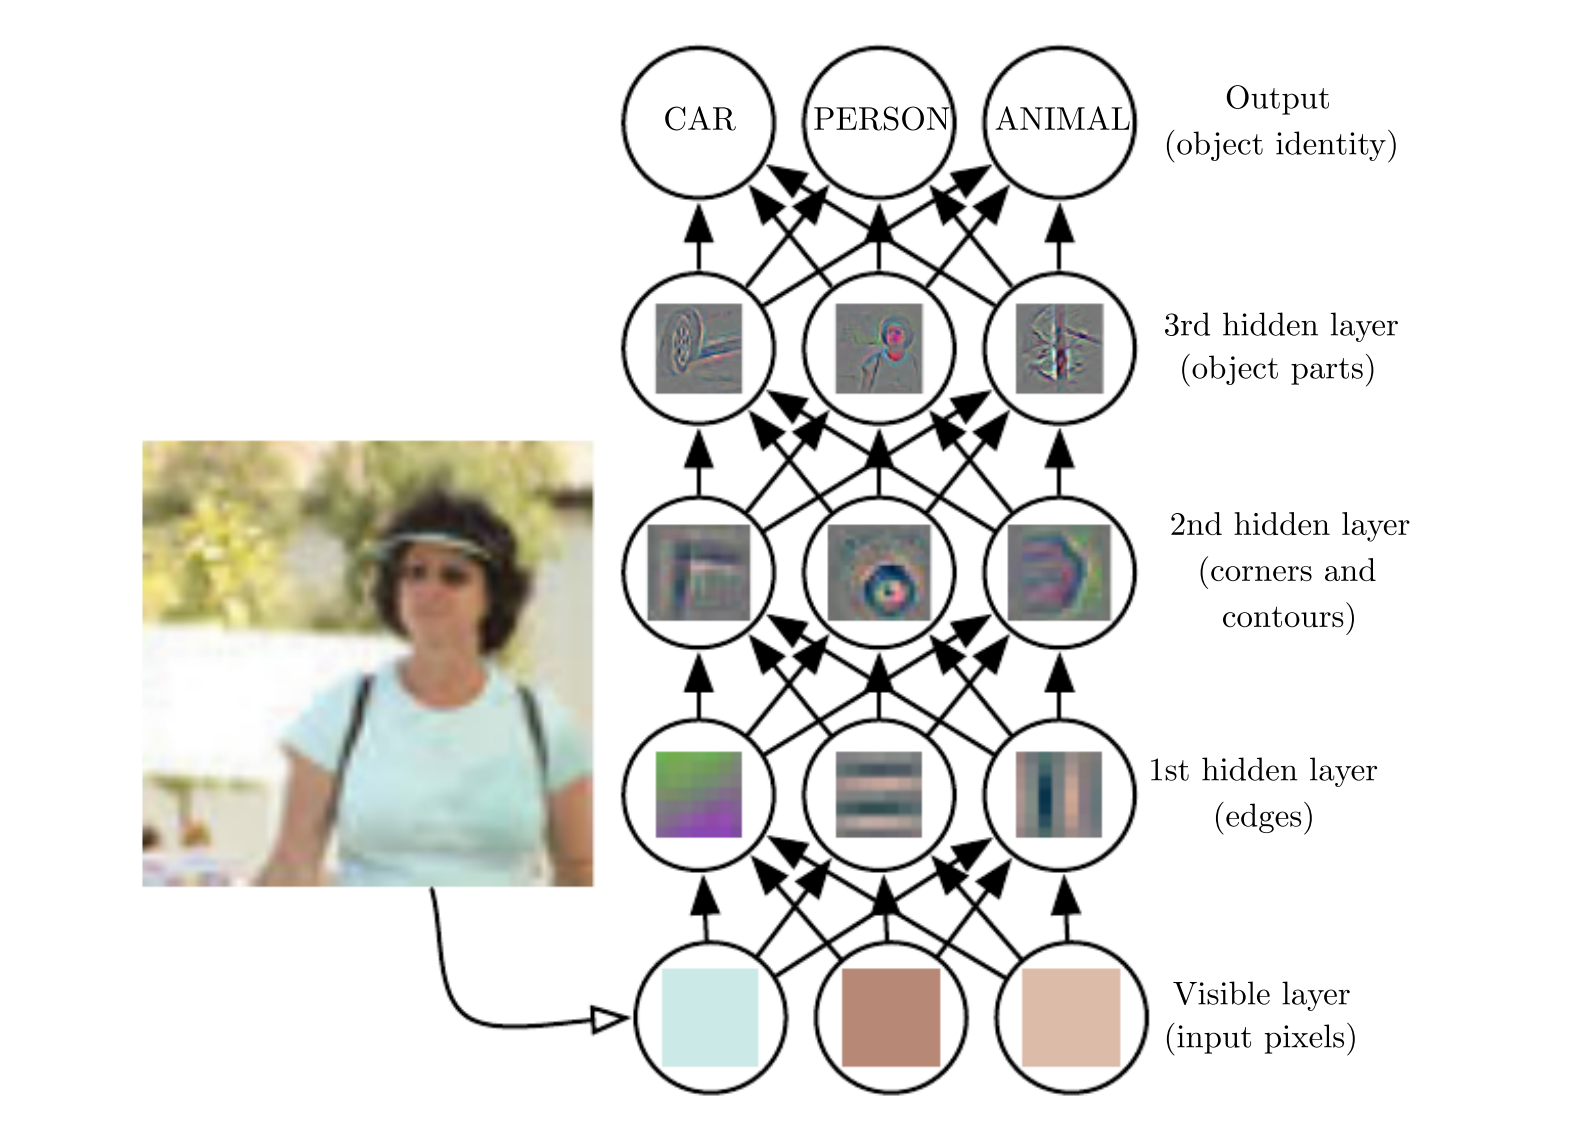
\includegraphics[width=12cm]{kapitel2/vision.png}
  \caption[Illustration eines Deep-Learning-Modells]{Illustration eines Deep-Learning-Modells aus \cite{IanGoodfellowYoshuaBengio2016} und \cite{Suah2017}: Ein Computer kann ohne weiteres das Bild in dieser Abbildung nicht erfassen, da es keine sensorischen Rohdaten verstehen kann. Das Bild in dieser Abbildung ist nur eine Sammlung von Pixelwerten. Die Funktionszuordnung von einem Satz von Pixeln zu einer Objektidentität ist sehr kompliziert.  Deep Learning löst diese Schwierigkeit, indem das gewünschte komplizierte \enquote{Mapping} in eine Reihe verschachtelter einfacher Mappings aufgeteilt wird, die jeweils durch eine andere Ebene des Modells beschrieben werden. Die Eingabe wird auf der \enquote{sichtbaren Ebene} (visible layer) dargestellt. Diese Schicht wird so genannt, weil sie die Variablen enthält, die wir beobachten können. Dann extrahieren eine Reihe \enquote{versteckter Ebenen} (hidden layer) zunehmend abstrakte Merkmale aus dem Bild. Diese Ebenen werden als \enquote{versteckt} bezeichnet, da ihre Werte nicht in den Daten angegeben sind. Stattdessen muss das Modell bestimmen, welche Konzepte zur Erklärung der Beziehungen in den beobachteten Daten nützlich sind. Angesichts der Pixel kann die erste Schicht Kanten nur leicht identifizieren, indem die Helligkeit benachbarter Pixel vergleicht. Angesichts der Beschreibung der Kanten durch die erste verborgene Ebene kann die zweite verborgene Ebene nach Ecken und erweiterten Konturen suchen. Angesichts der Beschreibung des Bildes durch die zweite verborgene Ebene in Bezug auf Ecken und Konturen kann die dritte verborgene Ebene ganze Teile bestimmter Objekte erkennen, indem bestimmte Konturen und Ecken gefunden werden. Schließlich kann diese Beschreibung des Bildes in Bezug auf die darin enthaltenen Objektteile verwendet werden, um die im Bild vorhandenen Objekte zu erkennen.}
  \label{Kap2:Vison}
\end{figure}

\section{Das Perzeptron}
Das Perzeptron kann ins deutsche mit dem Begriff der \enquote{Wahrnehmung} übersetzt werden. Das Perzeptron ist ein einfacher Algorithmus mit einem Eingabevektor $x$ mit $m$ Werten $(x_2, ..., x_m)$. Es wird oft wird als \enquote{Eingabe-Features} oder einfach als \enquote{Features} bezeichnet und zurückgegeben wird entweder eine $1$ \enquote{Ja} oder eine $0$ \enquote{Nein} (siehe Formel~\ref{Formel2_1}).

In Formel~\ref{Formel2_1}  ist $w$ ein Vektor welches das Gewicht darstellt, und $wx$ das Punktprodukt aus $\begin{array}{l}
    {\textstyle \sum ^{m}_{j=1}} w_{j} x_{j} \\
  \end{array}$, $b$ ist der Bias.
Aus $wx + b$ ist die Grenzhyperebene definiert, die die Position gemäß den $w$ und $b$ zugewiesenen Werten ändert.

\begin{equation}
  fx=\begin{cases}
    1 & wx+b >0   \\
    0 & ansonsten
  \end{cases}
  \label{Formel2_1}
\end{equation}

Mit anderen Worten, ist dies ein sehr einfacher, aber effektiver Algorithmus. Beispielsweise kann das Perzeptron bei drei Eingabemerkmalen  (Rot, Grün und Blau) unterscheiden, ob die Farbe weiß ist oder nicht. Es soll beachtet werden, dass das Perzeptron keine \enquote{Vielleicht}-Antwort ausdrücken kann. Es kann mit \enquote{Ja} (1) oder \enquote{Nein} (0) antworten. Das Perzeptron-Modell kann also benutzt werden, indem durch Anpassung von $w$ und $b$, das Modell \enquote{trainiert} wird.

\section{Bias}
Der Bias kann als Maß dafür vorgestellt werden, wie einfach es ist, das Perzeptron dazu zu bringen, um eine 1 auszugeben. Um es biologischer auszudrücken, ist der Bias ein Maß dafür, wie einfach es ist, das Perzeptron zum Feuern zu bringen. Für ein Perzeptron mit einem wirklich großen Bias ist es für das Perzeptron extrem einfach, eine 1 auszugeben. Wenn der Bias jedoch sehr negativ ist, ist es für das Perzeptron schwierig, eine 1 auszugeben \cite*[7]{Nielsen2015}.

\section{Mehrschichtiges Perzeptron}
In der Vergangenheit war \enquote{Perzeptron} der Name eines Modells mit einer einzigen linearen Schicht. Wenn es mehrere Schichten hat, wurde es daher als mehrschichtiges Perzeptron (Multi-layer perceptron / MLP) bezeichnet. Die Eingabe- und Ausgabeebene  ist von außen sichtbar, während alle anderen Ebenen in der Mitte ausgeblendet sind - daher der Name ausgeblendete Ebenen (hidden layers). In diesem Zusammenhang ist eine einzelne Schicht einfach eine lineare Funktion, und der MLP wird daher erhalten, indem mehrere einzelne Schichten nacheinander gestapelt werden (siehe Abbildung~\ref{Kap2:Multi}).

\begin{figure}[H]
  \centering
  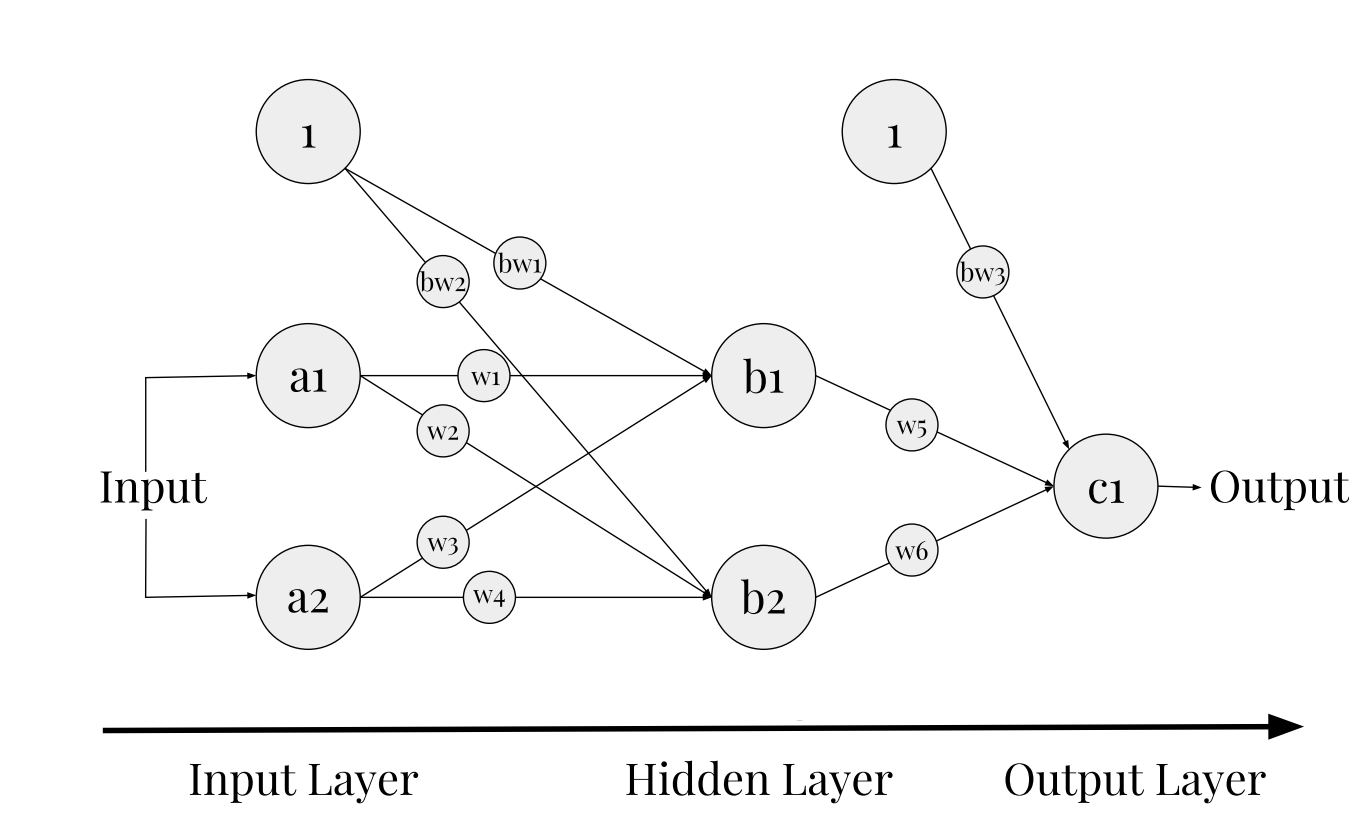
\includegraphics[width=12cm]{kapitel2/multilayer.png}
  \caption[Das mehrschichtige Perzeptron]{Ein Beispiel für ein mehrschichtiges Perzeptron in Anlehnung an \cite{Taylor2017}: Jeder Knoten in der ersten verborgenen Schicht empfängt eine Eingabe und \enquote{feuert} eine 0 oder 1 gemäß den Werten der zugehörigen linearen Funktion. Dann wird die Ausgabe der ersten verborgenen Schicht an die zweite Schicht übergeben, wo eine andere lineare Funktion angewendet wird, deren Ergebnisse an die endgültige Ausgabeschicht übergeben werden. Die letzte Schicht besteht nur aus einem einzelnen Neuron. Es ist interessant festzustellen, dass diese geschichtete Organisation vage der Organisation des menschlichen Sichtsystems ähnelt, wie zuvor besprochen.}
  \label{Kap2:Multi}
\end{figure}

Was sind die besten Entscheidungen für das Gewicht $w$ und den Bias $b$? Um diese Frage zu beantworten, wird nur ein einzelnes Neuron (ein einzelner Knoten) betrachtet.

Im Idealfall werden eine Reihe von Trainingsbeispielen bereitgestellt und der Computer muss das Gewicht $w$ und den Bias $b$ so einstellen, dass die in der Ausgabe erzeugten Fehler minimiert werden.

Um dies etwas konkreter zu machen, wird angenommen, dass es eine Reihe von Katzenbildern vorhanden sind und eine weitere separate Reihe von Bildern, die keine Katzen enthalten. Angenommen, jedes Neuron empfängt Eingaben vom Wert eines einzelnen Pixels in den Bildern. Während der Computer diese Bilder verarbeitet, möchten wir, dass unser Neuron seine Gewichte und seine Vorspannung so anpasst, dass immer weniger Bilder falsch erkannt werden.
Dieser Ansatz scheint sehr intuitiv zu sein, erfordert jedoch eine kleine Änderung der Gewichte (oder des Bias), um nur eine kleine Änderung der Ausgänge zu bewirken. Wenn wir einen großen Leistungssprung haben, können wir nicht progressiv lernen. Es wird gewünscht, wie ein \enquote{Kind} zu lernen, nach und nach. Das Perzeptron zeigt jedoch dieses \enquote{Stück für Stück}-Verhalten nicht. Ein Perzeptron gibt entweder eine 0 oder eine 1 zurück und das ist ein großer Sprung, der beim Lernen nicht hilft.


\section{Sigmoid-Neuron}
Das Verhalten des Perzeptron ist sehr  \enquote{uneben}, sodass ein \enquote{glatteres} nötig ist. Wir brauchen eine Funktion, die sich ohne Diskontinuität schrittweise von 0 auf 1 ändert. Mathematisch bedeutet dies, dass wir eine stetige Funktion benötigen, mit der wir die Ableitung berechnen können.

Dieses Problem kann überwunden werden, indem einen neuer Typ eines künstlichen Neurons eingeführt wird, der als Sigmoid-Neuron. Sigmoidneuronen ähneln Perzeptronen, sind jedoch so modifiziert, dass kleine Änderungen ihres Gewichts und ihres Bias nur eine geringe Änderung ihrer Leistung bewirken. Dies ist die entscheidende Tatsache, die es einem Netzwerk von Sigmoidneuronen ermöglicht, zu lernen \cite*[8]{Nielsen2015}.

Genau wie ein Perzeptron hat das Sigmoid-Neuron die Eingaben $x_1, x_2, ...$, aber anstatt nur 0 oder 1 zu sein, können diese Eingänge auch beliebige Werte zwischen 0 und 1 annehmen. Also zum Beispiel 0,123 welches eine gültige Eingabe für ein Sigmoid-Neuron ist. Ebenso wie ein Perzeptron hat das Sigmoid-Neuron Gewichte für jede Eingabe, $w_1, w_2, ...$ und einen Bias, $b$. Die Ausgabe ist jedoch nicht 0 oder 1, stattdessen ist es $\sigma$, $(wx + b)$, wobei $\sigma$ als Sigmoidfunktion bezeichnet wird und durch Formel~\ref{Formel2_2} definiert ist.

\begin{equation} \label{Formel2_2}
  \sigma (z) = \frac{1}{1+e^{-z}}
\end{equation}


\section{Aktivierungsfunktionen}
Ohne eine Aktivierungsfunktion (auch als Nichtlinearität bezeichnet) würde die dichte Schicht (dense layer) nuraus zwei linearen Operationen bestehen - einem Punktprodukt und einer Addition: $Ausgabe = Punkt (w, Eingabe) + b$. Die Schicht konnte also nur lineare Transformationen (affine Transformationen) der Eingabedaten lernen. Um Zugang zu einem viel umfangreicheren Hypothesenraum zu erhalten, wird eine Nichtlinearitäts- oder Aktivierungsfunktion benötigt \cite*[S. 72]{Chollet2017}. Es gibt weitaus mehr Aktivierungsfunktionen, als die in die in diesem Abschnitt beschriebenen. Es sollen hier nur die gängigsten 3 vorgestellt werden.

\subsection{Sigmoid}
Die Sigmoidfunktion wurde bereits mit der Formel~\ref{Formel2_2} definiert und in der Abbildung~\ref{Kap2:Sigmoid_plot} dargestellt, die Ableitung der Sigmoidfunktion ist in der Formel~\ref{Formel2_2Abl}. Sie hat kleine Ausgangsänderungen im Bereich (0, 1), wenn der Eingang im Bereich $(-\infty, \infty)$ variiert. Mathematisch ist die Funktion stetig. Ein Neuron kann das Sigmoid zur Berechnung der nichtlinearen Funktion $\sigma(z = wx + b)$ verwenden.
Wenn $z = wx + b$ sehr groß und positiv ist, dann wird $e^z \rightarrow 0$ also $\sigma(z) \rightarrow 1$, während wenn $z = wx + b$ sehr groß und negativ ist dann wird $e^{-z} \rightarrow 0$ also $\sigma(z) \rightarrow 0$. Mit anderen Worten, ein Neuron mit Sigmoidaktivierung hat ein ähnliches Verhalten wie das Perzeptron, aber die Änderungen sind allmählich und Ausgabewerte wie 0,54321 oder 0,12345 sind vollkommen legitim. In diesem Sinne kann ein Sigmoid-Neuron \enquote{vielleicht} antworten \cite*[10]{AntonioGuili;AmitaKapoor;SujitPal2019}.
\begin{figure}[H]
  \centering
  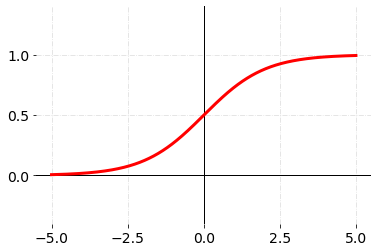
\includegraphics[width=8cm]{kapitel2/sig_plot.png}
  \caption[Darstellung der Sigmoid-Aktivierungsfunktion]{Darstellung der Sigmoid-Aktivierungsfunktion (eigene Darstellung)}
  \label{Kap2:Sigmoid_plot}
\end{figure}


\begin{equation} \label{Formel2_2Abl}
  \begin{array}{ c }
    \sigma '(z)\ =\ \frac{d}{dz}\left(\frac{1}{1+e^{-z}}\right) =\frac{1}{\left( 1+e^{-z}\right)^{-2}}\frac{d}{dz} =\left( e^{-z}\right) \ =\frac{e^{-z}}{\left( 1+e^{-z}\right)}\frac{1}{\left( 1+e^{-z}\right)} \ =  \\
    \\
    \frac{e^{-z} +1-1}{\left( 1+e^{-z}\right)}\frac{1}{\left( 1+e^{-z}\right)} =\left(\frac{\left( 1+e^{-z}\right)}{\left( 1+e^{-z}\right)} -\frac{1}{\left( 1+e^{-z}\right)}\right)\frac{1}{\left( 1+e^{-z}\right)} = \\
    \\
    \left( 1-\frac{1}{\left( 1+e^{-z}\right)}\right)\left(\frac{1}{\left( 1+e^{-z}\right)}\right) =\ (1-\sigma (z))\sigma (z)
  \end{array}
\end{equation}

\subsection{Tanh}
Die Tanh-Aktivierungsfunktion wird mit der Formel~\ref{Formel2_3} definiert. Sie hat ihre Ausgangsänderungen im Bereich (-1, 1). Sie hat eine Struktur, die der Sigmoid-Funktion sehr ähnlich ist. Der Vorteil gegenüber der Sigmoidfunktion besteht darin, dass ihre Ableitung steiler ist, was bedeutet, dass sie mehr Wert erhalten kann (vergleiche Abbildung~\ref{Kap2:Tanh_plot}). Für die Ableitung der Tanh-Aktivierungsfunktion gilt, $e^z = \frac{d}{dz}e^z$ und $e^{-z} = \frac{d}{dz}e^{-z}$, somit ist die Abletiung dieser Funktion in der Formel~\ref{Formel2_3Abl} angegeben.

\begin{equation} \label{Formel2_3}
  tanh(z) = \frac{e^{z}-e^{-z}}{e^{z}-e^{-z}}
\end{equation}

\begin{equation} \label{Formel2_3Abl}
  \begin{array}{ c }
    \frac{d}{dz} tanh( x) =\frac{\left( e^{z} +e^{-z}\right)\left( e^{z} +e^{-z}\right) -\left( e^{z} -e^{-z}\right)\left( e^{z} -e^{-z}\right)}{\left( e^{z} +e^{-z}\right)^{2}} = \\
    \\
    1-\frac{\left( e^{z} -e^{-z}\right)^{2}}{\left( e^{z} +e^{-z}\right)^{2}} \ =\ 1\ -tanh^{2}( z)
  \end{array}
\end{equation}

\begin{figure}[H]
  \centering
  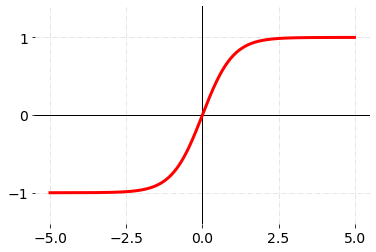
\includegraphics[width=8cm]{kapitel2/tanh_plot.png}
  \caption[Darstellung der Tanh-Aktivierungsfunktion]{Darstellung der Tanh-Aktivierungsfunktion (eigene Darstellung)}
  \label{Kap2:Tanh_plot}
\end{figure}

\subsection{ReLu}
Vor kurzem wurde eine sehr einfache Funktion namens ReLU (REctified Linear Unit) sehr beliebt, da sie dazu beiträgt, einige bei Sigmoiden beobachtete Optimierungsprobleme zu lösen \cite*[11]{AntonioGuili;AmitaKapoor;SujitPal2019}. Eine ReLU wird relativ einfach in und wird in der Formel~\ref{Formel2_4} definiert, die zugehörige Ableitungsfunktion ist in der Formel~\ref{Formel2_4Abl}. Wie in Abbildung~\ref{Kap2:ReLu_plot} zu sehen, ist die Funktion für negative Werte Null und wächst für positive Werte linear. Die ReLU ist relativ einfach zu implementieren (im Allgemeinen reichen drei Anweisungen aus), während das Sigmoid einige Größenordnungen mehr benötigt.

\begin{equation} \label{Formel2_4}
  f( x) \ =\ \begin{cases}
    0 & wenn\ x\  <\ 0    \\
    x & wenn\ x\  \geq\ 0 \\
  \end{cases}
\end{equation}

\begin{equation} \label{Formel2_4Abl}
  f'( x) \ =\ \begin{cases}
    1, & wenn\ x\  >\ 0 \\
    0, & sonst
  \end{cases}
\end{equation}

\begin{figure}[H]
  \centering
  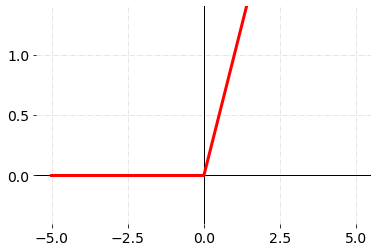
\includegraphics[width=8cm]{kapitel2/relu_plot.png}
  \caption[Darstellung der ReLu-Aktivierungsfunktion]{Darstellung der ReLu-Aktivierungsfunktion (eigene Darstellung)}
  \label{Kap2:ReLu_plot}
\end{figure}


\section{Optimierungsalgorithmen}
Die meisten Deep-Learning-Algorithmen beinhalten irgendeine Art von Optimierung. Optimierung bezieht sich auf die Aufgabe, eine Funktion $f(x)$ durch Ändern von $x$ entweder zu minimieren oder zu maximieren. Wir formulieren die meisten Optimierungsprobleme normalerweise in Bezug auf die Minimierung von $f(x)$. Die Maximierung kann über einen Minimierungsalgorithmus durch Minimieren von $-$$f(x)$ erreicht werden. Die Funktion, die wir minimieren oder maximieren möchten, wird als \enquote{objektive Funktion} oder \enquote{Kriterium} bezeichnet. Wenn wir es minimieren, können wir es auch als Kostenfunktion, Verlustfunktion oder Fehlerfunktion bezeichnen. Die Funktion $x^{*} = arg\ min\ f( x)$ ist eine solche Funktion.

    \begin{figure}[H]
      \centering
      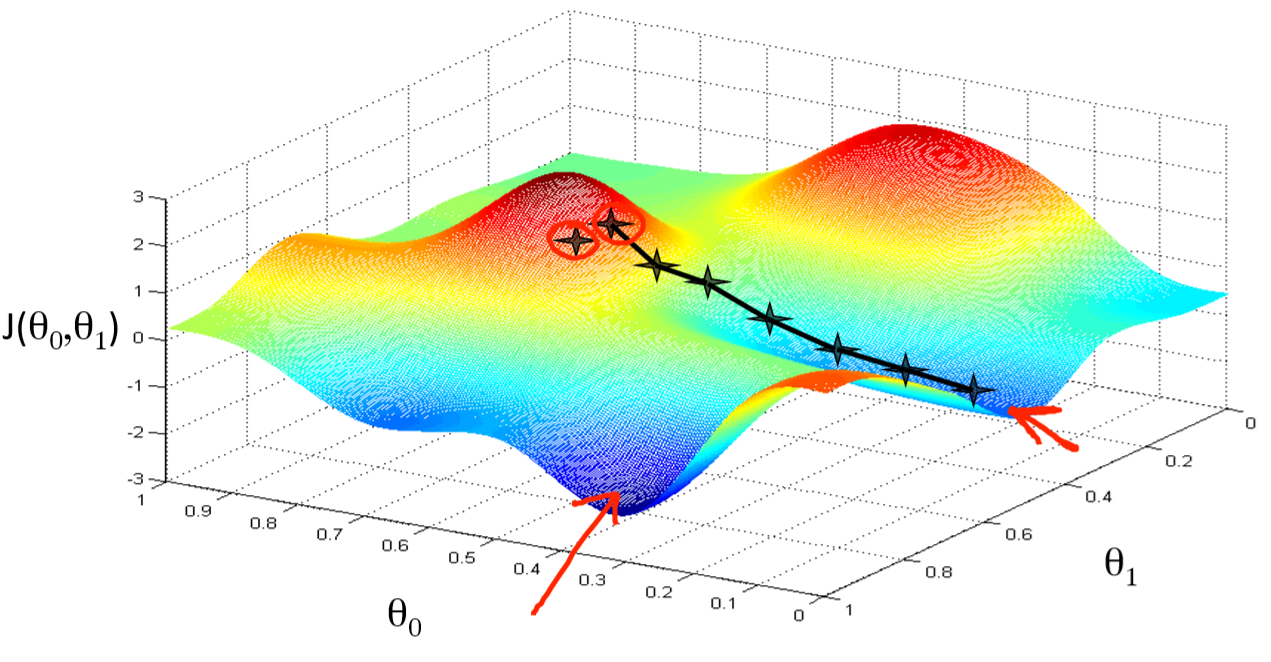
\includegraphics[width=14cm]{kapitel2/gradient.png}
      \caption[Der Gradientenabstieg]{Darstellung des Gradientenabstiegs, entnommen aus \cite*{IanGoodfellowYoshuaBengio2016}. Der Algorithmus nimmt die Ableitung der Funktion bis hin zum Minimum.}
      \label{Kap2:Grad}
    \end{figure}

    Beim Gradientenabstieg können wir uns die Qualität der Vorhersagen unseres Netzwerks als Landschaft vorstellen. Die Hügel stellen Orte (Parameterwerte oder Gewichte) dar, die viele Vorhersagefehler verursachen. Täler repräsentieren Orte mit weniger Fehlern. Wir wählen einen Punkt in dieser Landschaft, an dem wir unser anfängliches Gewicht platzieren möchten. Wir können dann das Anfangsgewicht basierend auf dem Domänenwissen auswählen (wenn wir ein Netzwerk trainieren, um eine Blumenart zu klassifizieren, wissen wir, dass die Blütenblattlänge wichtig ist, die Farbe jedoch nicht). Wenn wir das Netzwerk die ganze Arbeit machen lassen, wählen wir die Anfangsgewichte möglicherweise zufällig aus. Der Zweck besteht darin, dieses Gewicht so schnell wie möglich bergab in Bereiche mit geringerem Fehler zu bewegen. Ein Optimierungsalgorithmus wie der Gradientenabstieg kann die tatsächliche Neigung der Hügel in Bezug auf jedes Gewicht erfassen. Das heißt, es weiß, in welche Richtung es geht. Der Gefälle-Abstieg misst die Steigung (die durch eine Gewichtsänderung verursachte Fehleränderung) und nimmt das Gewicht einen Schritt in Richtung Talboden \cite*[34]{Patterson2019} (siehe Abbildung Abbildung~\ref{Kap2:Grad}).

    % \paragraph{Lernrate}
    % Die Größe des Lernens, also wird als Lernrate bezeichnet. Mit einer hohen Lernrate können wir mit jedem Schritt mehr abdecken, aber wir riskieren, den tiefsten Punkt zu überschreiten, da sich die Neigung des Hügels ständig ändert. Mit einer sehr niedrigen Lernrate können wir uns sicher in Richtung des negativen Gradienten bewegen, da wir ihn so häufig neu berechnen. Eine niedrige Lernrate ist genauer, aber die Berechnung des Gradienten ist zeitaufwändig, sodass wir sehr lange brauchen, um auf den Grund zu gehen.


    Es gibt drei Varianten des Gradientenabfalls, die sich darin unterscheiden, wie viele Daten wir zur Berechnung des Gradienten der Zielfunktion verwenden. Abhängig von der Datenmenge machen wir einen Kompromiss zwischen der Genauigkeit der Parameteraktualisierung und der Zeit, die für die Durchführung einer Aktualisierung benötigt wird \cite*{Ruder2016}. In den nächsten beiden Abschnitten werden zwei Varianten vorgestellt.

    \subsection{Batch Gradientenabstiegsverfahren}
    Der Standart Gradientenabstiegsverfahren, auch Batch-Gradientenabstiegsverfahren genannt, berechnet den Gradienten der Kostenfunktion zu den Parametern $\theta$ für den gesamten Trainingsdatensatz.


    \begin{equation} \label{FormelGradBatch}
      \theta = \theta - \eta \cdot \nabla_{\theta}J(\theta)
    \end{equation}

    Da der gesamte Datensatz berechnet werden muss, um nur eine Aktualisierung durchzuführen, kann der Batch-Gradientenabstieg sehr langsam sein und ist für Datensätze, die nicht in den Speicher passen, nicht zu handhaben. Der Batch-Gradientenabstieg ermöglicht es auch nicht, das Modell mit neuen Beispielen im laufenden Betrieb zu aktualisieren \cite*{Ruder2016}.

    \subsection{Stochastische Gradientenabstiegsverfahren}

    Im Gegensatz dazu führt der stochastische Gradientenabstiegsverfahren (SGD) eine Parameteraktualisierung für jedes Trainingsbeispiel durch. Der Batch-Gradientenabstieg führt redundante Berechnungen für große Datenmengen durch, da Gradienten für ähnliche Beispiele vor jeder Parameteraktualisierung neu berechnet werden. Der Stochastische Gradientenabstiegsverfahren beseitigt diese Redundanz, indem jeweils ein Update durchgeführt wird. Es ist daher in der Regel viel schneller und kann auch beim laufenden Lernen verwendet werden \cite*{Ruder2016}.

    \begin{equation} \label{FormelGradStoch}
      \theta = \theta - \eta \cdot \nabla_{\theta}J(\theta;x^{(i)};y^{(i)})
    \end{equation}



    \section{Lernrate im Deep Learning}
    Die Lernrate beeinflusst den Betrag, um den die Parameter während der Optimierung angepasst werden, um den Fehler des neuronalen Netzwerks zu minimieren. Es ist ein Koeffizient, der die Größe der Schritte (Aktualisierungen) skaliert, die ein neuronales Netzwerk auf seinen Parameter (Vektor $x$) ausführt, wenn es den Verlustfunktionsraum durchquert. Ein großer Lernratenkoeffizient (z. B. 1) lässt die Parameter Sprünge machen, und kleine (z. B. 0,00001) lassen ihn langsam voranschreiten. Im Gegensatz dazu sollten kleine Lernraten letztendlich zu einem Fehlerminimum führen (es kann eher ein lokales als ein globales Minimum sein), aber sie können sehr lange dauern und die Belastung eines bereits rechenintensiven Prozesses erhöhen  \cite*[77]{Patterson2019}.


    \begin{figure}[H]
      \centering
      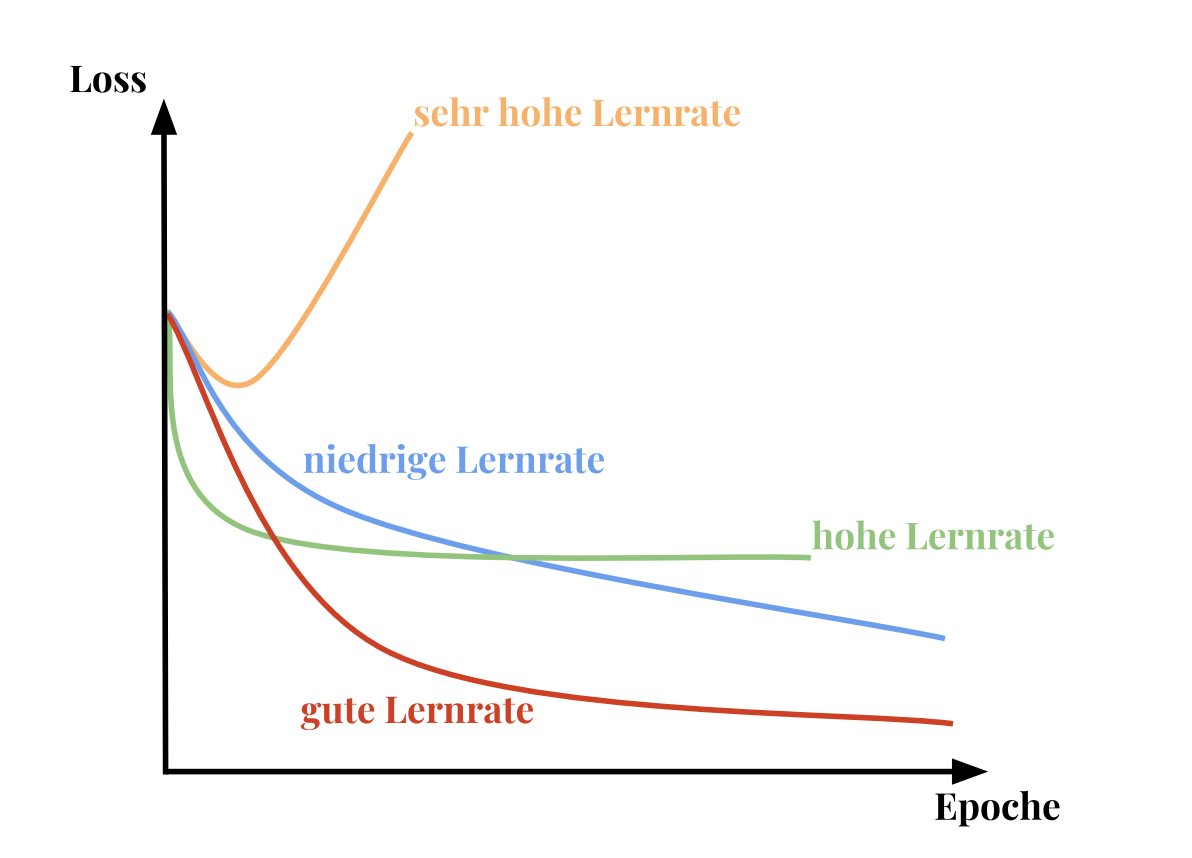
\includegraphics[width=10cm]{kapitel2/learnrate.png}
      \caption[Einfluss der Lernrate auf den Verlust]{Vergleich unterschiedlicher Lernraten und deren Effekt auf den Verlust. Bei niedrigen Lernraten ist eine \enquote{lineare} Verbesserungen zu sehen. Mit hohen Lernraten werden sie exponentieller. Höhere Lernraten verringern den Verlust schneller, bleiben jedoch bei schlechteren Verlustwerten hängen (grüne Linie). Dies liegt daran, dass die Optimierung zu viel \enquote{Energie} enthält und die Parameter \enquote{chaotisch herumspringen} und sich nicht an einem Ort in der Optimierungslandschaft niederlassen können (in Anlehnung an \cite*{StanfordUniversityCoursecs231n2018}). }
      \label{Kap2:Lern}
    \end{figure}

    \section{Unteranpassung und Überanpassung}
    Optimierungsalgorithmen versuchen zunächst, das Problem der Unteranpassung \enquote{Underfitting} zu lösen. Das heißt, eine Linie zu nehmen, die sich den Daten nicht gut annähert, und sie besser an die Daten heranzuführen. Eine gerade Linie, die über ein gekrümmtes Streudiagramm schneidet, wäre ein gutes Beispiel für eine Unteranpassung, wie in Abbildung~\ref{Kap2:OverUnder} dargestellt. Wenn die Linie zu gut zu den Daten passt, haben wir das gegenteilige Problem, das als Überanpassung \enquote{Overfitting} bezeichnet wird \cite*[27]{Patterson2019}.

    \begin{figure}[H]
      \centering
      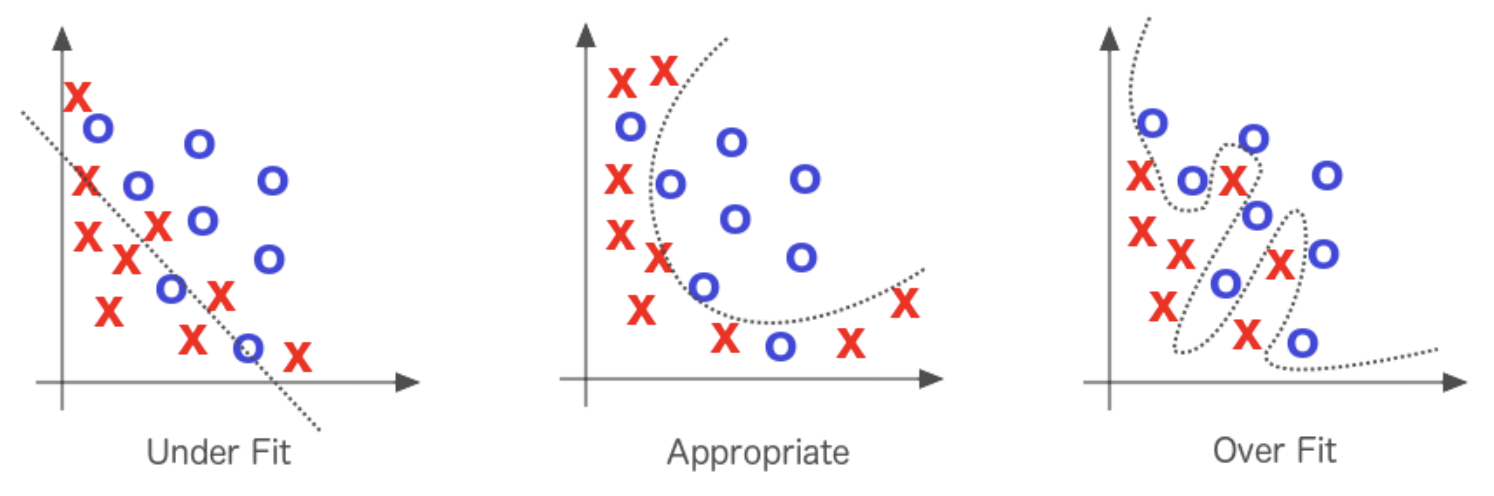
\includegraphics[width=10cm]{kapitel2/overundefit.png}
      \caption[Vergleich der Unteranpassung mit der Überanpassung]{Die Abbildung vergleicht die Überanpassung mit der Unteranpassung. Die einzelnen Punkte passen sich dem trainierten Model zu sehr an, der Verlust wird also so klein, dass die das Modell nicht mehr zuverlässige Ergebnisse liefern kann. Dies ist darauf zurückzuführen, dass das Modell \enquote{zu viel} aus dem Trainingsdatensatz gelernt hat. Unteranpassung ist der Fall, wenn das Modell aus den Trainingsdaten \enquote{nicht genug gelernt} hat, was zu einer geringen Verallgemeinerung und unzuverlässigen Vorhersagen führt (Grafik entnommen aus \cite*[27]{Patterson2019}). }
      \label{Kap2:OverUnder}
    \end{figure}

    \section{Regularisierung}
    Die Regularisierung hilft bei den Auswirkungen von außer Kontrolle geratenen Parametern, indem verschiedene Methoden verwendet werden, um die Parametergröße im Laufe der Zeit zu minimieren. Der Hauptzweck der Regularisierung besteht darin, die Überanpassung zu kontrollieren \cite*[79]{Patterson2019}.

    Ein zentrales Problem beim maschinellen Lernen besteht darin, einen Algorithmus zu erstellen, der nicht nur bei den Trainingsdaten, sondern auch bei neuen Eingaben eine gute Leistung erbringt. Viele beim maschinellen Lernen verwendete Strategien sind explizit darauf ausgelegt, den Testfehler zu reduzieren, möglicherweise auf Kosten eines erhöhten Trainingsfehlers. Diese Strategien werden zusammen als Regularisierung bezeichnet. Tatsächlich war die Entwicklung effektiverer Regularisierungsstrategien eine der wichtigsten Forschungsanstrengungen auf diesem Gebiet, in den folgenden Abschnitten sollen sollen einige Strategien dargestellt werden. Regularisierung kann schließlich definiert werden als \enquote{jede Änderung, die wir an einem Lernalgorithmus vornehmen, um dessen Generalisierungsfehler, aber nicht seinen Trainingsfehler zu reduzieren} \cite*[228]{IanGoodfellowYoshuaBengio2016}.

    \subsection{Early Stopping}
    Wenn große Modelle mit trainiert werden, um eine bestimmte Aufgabe lösen, wird häufig festgestellt, dass der Trainingsfehler mit der Zeit stetig abnimmt, der Fehler des Validierungssatzes jedoch wieder zunimmt. Dies bedeutet, dass ein Modell mit einem besseren Validierungssatzfehler (und damit  einem besseren Testsatzfehler) erhalten werden kann, indem zu dem Zeitpunkt mit dem niedrigsten Validierungssatzfehler zur Parametereinstellung zurückgekehrt wird. Jedes Mal, wenn sich der Fehler im Validierungssatz verbessert, wird eine Kopie der Modellparameter gespeichert. Wenn der Trainingsalgorithmus beendet wird, wird diese Parameter anstelle der neuesten Parameter zurückgegeben. Diese Strategie wird als Early Sopping \enquote{frühes Stoppen} bezeichnet. Es ist wahrscheinlich die am häufigsten verwendete Form der Regularisierung. Seine Popularität ist sowohl auf seine Wirksamkeit als auch auf seine Einfachheit zurückzuführen \cite*[246]{IanGoodfellowYoshuaBengio2016}.


    \subsection{Dropout}
    Eine weitere Strategie um Überanpassung zu vermeiden wird in \cite*{Srivastava2014} dargestellt. Dropout bietet eine rechnerisch kostengünstige, aber leistungsstarke Methode zur Regularisierung dar. Es ist das aufteilen von mehreren Ensembles großer Netzwerke. Es wird also ein Ensemble, welches aus mehreren Subnetzwerken (sub-networks) gebildet wird \cite*[258]{IanGoodfellowYoshuaBengio2016}.



    \begin{figure}[H]
      \centering
      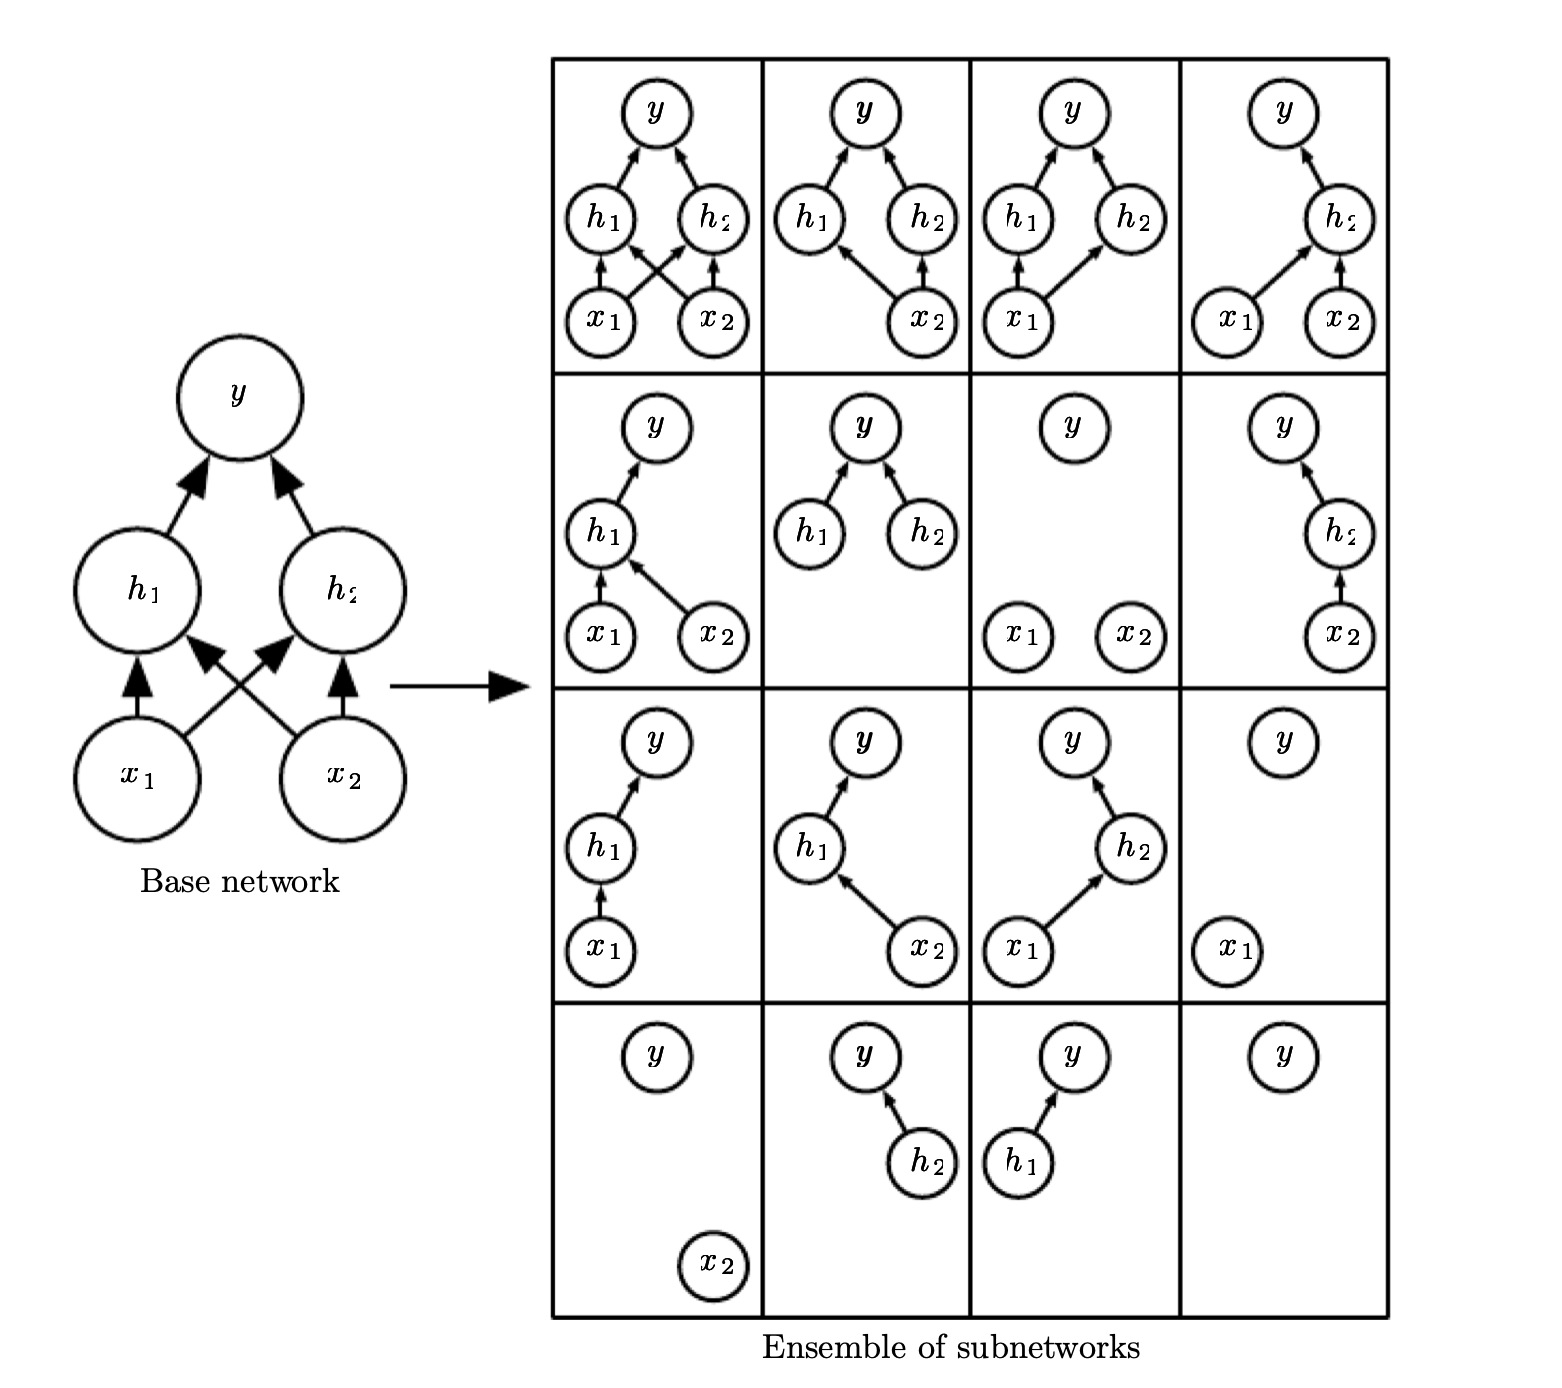
\includegraphics[width=10cm]{kapitel2/dropout.png}
      \caption[Basis-Netzwerks und Ensemble im Vergleich]{Dropout trainiert ein Ensemble. Ein Ensemble besteht aus allen Teilnetzwerken. Es wird durch das entfernen von Einheiten aufgebaut. Das Ensemble besteht aus 16 Teilmengen, aus den vier Einheiten des Basis-Netzwerks. Die 16 Subnetze werden durch das Löschen verschiedener Teilmengen von Einheiten aus dem ursprünglichen Netzwerk gebildet (entnommen aus \cite*[260]{IanGoodfellowYoshuaBengio2016}).}
      \label{Kap2:Dropout}
    \end{figure}

    \subsection{L1 und L2}
    Eine weitere Strategie der Regularisierung ist die Modifikation der L1 und L2 Gewichte. Manchmal müssen wir die Größe eines Vektors messen. Beim Deep Learning wird die Größe von Vektoren mit einer Funktion, die als \enquote{Norm} bezeichnet wird \cite*[39]{IanGoodfellowYoshuaBengio2016}. Formal ist die $L^p$ gegeben als:

    \begin{equation} \label{FormelNorm2}
      \Vert x\Vert \ =\ \left(\sum _{i}\bigr| x_{i}\bigr|^{p}\right)^{\frac{1}{p}}.
    \end{equation}

    Normen, einschließlich der $L^p$-Norm, sind Funktionen, die Vektoren auf nicht negative Werte abbilden. Auf einer intuitiven Ebene misst die Norm eines Vektors $x$ den Abstand vom Ursprung zum Punkt $x$. Die $L^2$-Norm mit $p = 2$ ist als euklidische Norm bekannt. Es ist der euklidische Abstand vom Ursprung zum Punkt $x$. Die $L^2$-Norm wird beim maschinellen Lernen häufig verwendet, sie wird einfach als $\Vert x\Vert$ bezeichnet, wobei der Index 2 weggelassen wird \cite*[39]{IanGoodfellowYoshuaBengio2016}.

    Wenn zwischen Elementen zu unterscheiden werden soll, die genau Null sind, und Elementen, die klein, aber ungleich Null sind wird eine Funktion angewendet, die an allen Standorten mit der gleichen Geschwindigkeit wächst, aber die mathematische Einfachheit beibehält: die L1-Norm. Die $L^1$-Norm kann vereinfacht werden als:

    \begin{equation} \label{FormelNorm1}
      \Vert x\Vert 1\ =\ \sum _{i}\bigr| x_{i}\bigr|.
    \end{equation}

    Die $L^2$-Norm wird üblicherweise beim maschinellen Lernen verwendet, wenn der Unterschied zwischen Null- und Nicht-Null-Elementen sehr wichtig ist \cite*[40]{IanGoodfellowYoshuaBengio2016}.


    \section{Verlustfunktion und Kreuzentropie}
    \subsection{Verlustfunktionen}
    Innerhalb eines neuronalen Netzwerks wandelt eine Verlustfunktion alle möglichen Fehler, in eine Zahl um, die den Gesamtfehler des Netzwerks darstellt. Im Wesentlichen ist es ein Maß dafür, wie falsch ein Netzwerk ist. Auf einer technischeren Ebene werden ein Ereignis oder Werte einer oder mehrerer Variablen einer reellen Zahl zugeordnet. Diese reelle Zahl stellt  den \enquote{Verlust} oder die \enquote{Kosten} dar, die mit dem Ereignis oder den Werten verbunden sind \cite*[61-62]{Taylor2017}.

    Das Neuron durch lern dadurch, indem es den Gewicht und den Bias mit einer Rate ändert, die durch die partiellen Ableitungen der Kostenfunktion $\partial$$C$/$\partial$$w$ und $\partial$$C$/$\partial$$b$ bestimmt wird. Zu sagen, dass  das \enquote{Lernen langsam ist}, ist also dasselbe wie zu sagen, dass diese partiellen Ableitungen klein sind. Die Herausforderung besteht darin zu verstehen, warum sie klein sind. Um dies zu verstehen, berechnen wir die partiellen Ableitungen \cite*[61]{Nielsen2015}. Gegeben sei die quadratische Verlustfunktion:

    \begin{equation} \label{Formel2_5}
      C=\frac{( y-a)^{2}}{2},
    \end{equation}

    dabei ist $a$ die Ausgabe des Neurons, wenn die Trainingseingabe $x = 1$ ist, und $y = 0$ die entsprechende gewünschte Ausgabe. Um dies in Bezug auf Gewicht und Bias expliziter zu schreiben, sei daran erinnert, dass $a = \sigma(z)$ ist, wobei $z = wx + b$ ist. Es ergeben sich durch die Anwendung der Kettenregel folgende Gleichungen:

    \begin{equation} \label{Formel2_6}
      \frac{\partial C}{\partial w} =( a-y) \sigma '( z) x=a\sigma '( z)
    \end{equation}

    \begin{equation} \label{Formel2_7}
      \frac{\partial C}{\partial b} =( a-y) \sigma '( z) =a\sigma '( z).
    \end{equation}

    Aus der Abbildung~\ref{Kap2:Sigmoid_plot} ist die Kurve der Sigmoidfunktion zu sehen, welches. Die Kurve wird sehr flach, wenn der Ausgang des Neurons nahe bei 1 liegt, und daher wird $\sigma'(z)$ sehr klein. Die Gleichungen~\ref{Formel2_6} und ~\ref{Formel2_7} sagen uns dann, dass $\partial$$C$/$\partial$$w$  und  $\partial$$C$/$\partial$$b$ sehr klein werden. Dies ist der Grund warum das lernen langsamer wird.

  \subsection{Kreuzentropie}
  Nach \cite*[62]{Nielsen2015} kann die Lernverlangsamung gelöst werden, indem die quadratischen Verlustfunktion durch eine andere Verlustfunktion ersetzt wird. Diese Funktion wird als als Kreuzentropie bezeichnet. Die Abbildung~\ref{Kap2:Entropie} zeigt die Kreuzentropie mit mehreren Eingabevariablen und entsprechenden Gewichten und dem Bias. Die Ausgabe des Neurons ist $a = \sigma(z)$, wobei $z =  \sum _{j} w_{j} b_{j} + b$ ist, die gewichtete Summe des Inputs. Wir definieren die Kreuzentropiekostenfunktion für dieses Neuron durch:

  \begin{equation} \label{Formel2_8}
    C=\ -\frac{1}{n}\sum _{x}[ y\ ln\ a\ +\ ( 1-y) \ ln( 1-a)]
  \end{equation}

  wobei $n$ die Gesamtzahl der Trainingselemente darstellt. Die Summe gibt die entsprechende gewünschte Ausgabe $x$ und $y$ über alle Trainingseingaben an. Zusammenfassend ist die Kreuzentropie positiv und tendiert gegen Null, wenn das Neuron
  \enquote{besser} wird in der Berechnung der gewünschten Ausgabe $y$ für alle Trainingseingaben $x$.  Die entropieübergreifende Kostenfunktion hat jedoch den Vorteil, dass sie im Gegensatz zu den quadratischen Kosten das Problem der Verlangsamung des Lernens vermeidet. Um dies zu sehen, berechnen wir die partielle Ableitung der Kreuzentropiekosten in Bezug auf die Gewichte \cite*[63]{Nielsen2015}.

  \begin{gather} \label{Formel2_9}
    \frac{\partial C}{\partial w_{j}} =-\frac{1}{n}\sum _{x}\left(\frac{y}{\sigma ( z)} -\frac{1-y}{1-\sigma ( z)}\right)\frac{\partial \sigma }{\partial w_{j}} = \notag\\
    \notag\\
    -\frac{1}{n}\sum _{x}\left(\frac{y}{\sigma ( z)} -\frac{1-y}{1-\sigma ( z)}\right) \sigma '( z) x_{j} \notag\\
  \end{gather}

  \begin{equation} \label{Formel2_10}
    \frac{\partial C}{\partial w_{j}} \ =\ \frac{1}{n}\sum _{x}\frac{\sigma '( z) x_{j}}{\sigma ( z)( 1-\sigma ( z))}( \sigma ( z) -y)
  \end{equation}

  \begin{equation} \label{Formel2_11}
    \frac{\partial C}{\partial w_{j}} \ =\ \frac{1}{n}\sum _{x} x_{j}( \sigma ( z) -y)
  \end{equation}


  Die Gleichungen~\ref{Formel2_9}, ~\ref{Formel2_10} und ~\ref{Formel2_11} zeigen dass die Geschwindigkeit, mit der das Gewicht $w$  lernt, durch $\sigma(z) - y$ gesteuert wird, also durch den Fehler in der Ausgabe. Je größer der Fehler wird, desto schneller lernt das Neuron. Dies ist genau das ein gewünschtes Verhalten. Insbesondere wird die Lernverlangsamung vermieden, die durch den Term $\sigma'(z)$ in der analogen Gleichung für die quadratischen Kostenfunktion~\ref{Formel2_6} verursacht wird. Wenn wir die Kreuzentropie verwenden, wird der Term $\sigma'(z)$ aufgehoben, und wir brauchen uns keine Sorgen mehr darüber zu machen, dass er klein ist. Diese Aufhebung ist das besondere, das durch die Kreuzentropie-Kostenfunktion gewährleistet wird \cite[63-64]{Nielsen2015}.

  Analog zur Gleichung\label{Formel2_9}, \label{Formel2_10} und \label{Formel2_11} ergibt die Berechnung für den Bias folgende Gleichung:

  \begin{equation}
    \frac{\partial C}{\partial b} \ =\ \frac{1}{n}\sum _{x}( \sigma ( z) -y).
  \end{equation}

  \begin{figure}[H]
    \centering
    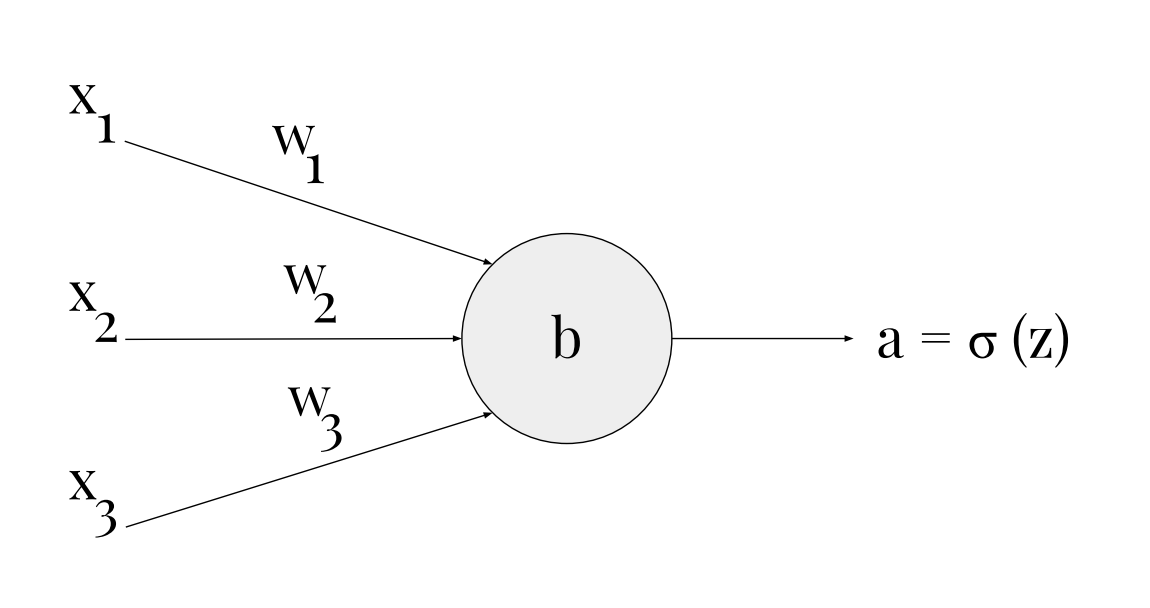
\includegraphics[width=8cm]{kapitel2/entropie.png}
    \caption[Darstellung der Kreuzentropie am beispiel eines Neurons]{Das Neuron wird mit 3 Eingabewerten $(x_1, x_2, x_3)$ den dazugehörigen Gewichten $(W_1, W_2, W_3)$ trainiert. Der Bias ist durch $b$ angegeben und die Ausgabe mit $a = \sigma(z)$ (in Anlehnung an \cite*{Nielsen2015})}
    \label{Kap2:Entropie}
  \end{figure}

  \section{Convolutional Neural Network}
  Convolutional Neural Networks (CNNs) arbeiten mit gitterstrukturierten Eingaben, die in lokalen Regionen des Netzes starke räumliche Abhängigkeiten aufweisen. Das offensichtlichste Beispiel für gitterstrukturierte Daten ist ein zweidimensionales Bild. Diese Art von Daten weist auch räumliche Abhängigkeiten auf, da benachbarte räumliche Orte in einem Bild häufig ähnliche Farbwerte der einzelnen Pixel aufweisen. Eine zusätzliche Dimension erfasst die verschiedenen Farben, wodurch ein dreidimensionales Eingabevolumen entsteht. Daher weisen die Merkmale in einem CNN Abhängigkeiten untereinander auf, die auf räumlichen Abständen beruhen. Andere Formen von sequentiellen Daten wie Text, Zeitreihen und Sequenzen können ebenfalls als Sonderfälle von Daten mit Gitterstruktur mit verschiedenen Arten von Beziehungen zwischen benachbarten Elementen betrachtet werden. Die überwiegende Mehrheit der Anwendungen von CNNs konzentriert sich auf Bilddaten, obwohl man diese Netze auch für alle Arten von zeitlichen, räumlichen und raumzeitlichen Daten verwenden kann. Ein wichtiges definierendes Merkmal von CNNs ist eine Operation, die als Faltung (convolution) bezeichnet wird. \cite*[315-316]{Aggarwal2018}.

  \subsection{Architektur}
  In CNNs sind mehrere Schichten miteinander verbunden und jeder Schicht hat  Gitterstruktur. Die Bezihungen zwischen den Schichten werden von einer Schicht zur nächsten vererbt, da jeder Merkmalswert auf einem kleinen lokalen Bereich aus der vorherigen Schicht basiert. Es ist wichtig, diese räumlichen Beziehungen zwischen den Gitterzellen aufrechtzuerhalten, da die Faltungsoperation und die Transformation zur nächsten Schicht von diesen Beziehungen abhängen. Jede Schicht im Faltungsnetzwerk ist eine dreidimensionale Gitterstruktur mit einer Höhe, Breite und Tiefe. Die Tiefe einer Schicht in einem Faltungsnetzwerk ist nicht die Tiefe des Netzwerks selbst. Das Wort \enquote{Tiefe} bezieht sich auf die Anzahl der Kanäle in jeder Ebene, z. B. die Anzahl der Primärfarbkanäle (z. B. Blau, Grün und Rot) im Eingabebild \cite*[318]{Aggarwal2018}.

  Ein ConvNet besteht aus Ebenen. Ein einfaches ConvNet ist eine Folge von Schichten, und jede Schicht eines ConvNet wandelt eine Schicht durch eine differenzierbare Funktion in ein anderes um. Es wird dabei drei Arten von Schichten geben um ein ConvNet Architekturen zu bauen: Faltungs-Schicht , Pooling-Schicht und die vollständig verbundene Schicht \cite*{StanfordUniversityCoursecs231n2018a}.

  \begin{figure}[H]
    \centering
    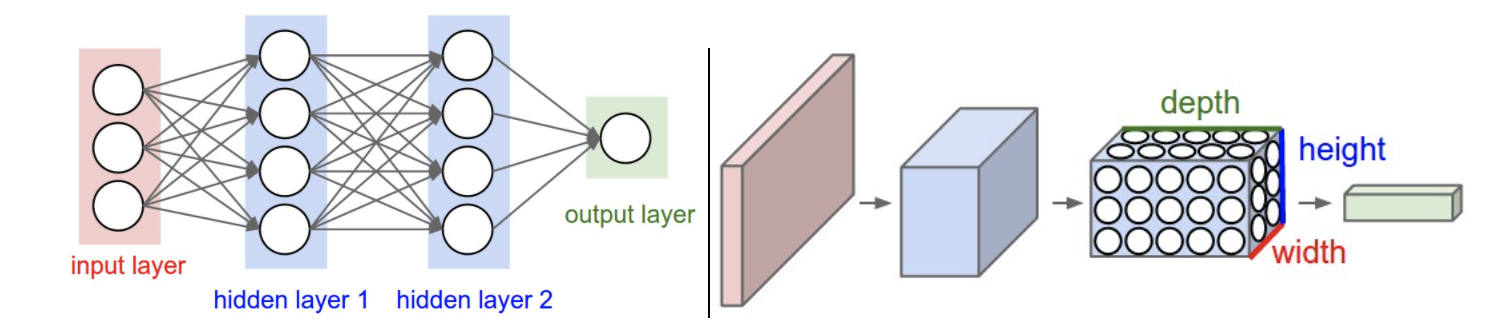
\includegraphics[width=13cm]{kapitel2/conv.png}
    \caption[Vergleich eines NN mit einem CNN]{Links: Ein reguläres 3-Schicht-Neuronales Netz. Rechts: Ein ConvNet ordnet seine Neuronen in drei Dimensionen (Breite, Höhe, Tiefe) an, wie in einer der Ebenen dargestellt. Jede Schicht eines ConvNet wandelt das 3D-Eingangsvolumen in ein 3D-Ausgangsvolumen von Neuronenaktivierungen um. In diesem Beispiel enthält die rote Eingabeebene das Bild, sodass seine Breite und Höhe den Abmessungen des Bildes entsprechen. Die \enquote{Tiefe} sind die 3 Farbkanäle (rot, grün, blau) aus \cite*{StanfordUniversityCoursecs231n2018a}.}
    \label{Kap2:Conv}
  \end{figure}

  % Im folgenden werden die einzelnen Elemente einer CNN-Architektur vorgestellt, welches einen Bild als Eingabe hat:

  % \begin{itemize}
  %   \item Eingabe: Enthält die Rohpixelwerte des Bildes, in diesem Fall ein Bild mit einer Breite von 32, einer Höhe von 32 und drei Farbkanälen R, G, B.
  %   \item Die CONV-Schicht: Berechnet die Ausgabe von Neuronen, die mit lokalen Regionen in der Eingabe verbunden sind, wobei jede ein Punktprodukt zwischen ihren Gewichten und einer kleinen Region berechnet, mit der sie im Eingabevolumen verbunden sind. Dies kann zu einem \enquote{Volumen} von [32x32x12] führen, wenn wir uns für die Verwendung von 12 Filtern entschieden haben.
  %   \item Die RELU-Ebene: Wendet eine elementweise Aktivierungsfunktion an, z. B. die maximale $(0, x)$ Schwellwertbildung bei Null. Dadurch bleibt die Größe des Volumes unverändert ([32x32x12]).
  %   \item Die POOL-Ebene: Führt einen \enquote{Downsampling-Vorgang} entlang der räumlichen Abmessungen (Breite, Höhe) durch, was zu einem Volumen von [16x16x12] führt.
  %   \item Die Vollständig verbunde Schicht: Berechnet die Klassenbewertungen, was zu einem Volumen der Größe [1 × 1 × 10] führt, wobei jede der 10 Zahlen einer Klassenbewertung entspricht \cite*{StanfordUniversityCoursecs231n2018a}.
  % \end{itemize}

  \subsection{Convolutional Layer}

  Die Parameter der CONV-Schicht bestehen aus einer Reihe von lernbaren Filtern. Jedes dieser Filter ist räumlich klein (Breite und Höhe), erstreckt sich jedoch über die gesamte Tiefe des Eingangsvolumens. Beispielsweise könnte ein typischer Filter auf einer ersten Schicht eines ConvNet die Größe 5 × 5 × 3 haben (d. H. 5 Pixel Breite und Höhe und 3, weil Bilder die Tiefe 3 haben, die Farbkanäle). Während des Vorwärtsdurchlaufs wird jedes der Filter über die Breite und Höhe des Eingangsvolumens gefaltet und es werden die Punktprodukte zwischen den Einträgen des Filters und dem Eingang an einer beliebigen Position berechnet. Wenn der Filter über die Breite und Höhe des Eingangsvolumens gefaltet wird, wird eine zweidimensionale Aktivierungskarte erstellt, die die Antworten dieses Filters an jeder räumlichen Position angibt. Intuitiv lernt das Netzwerk Filter, die aktiviert werden, wenn sie eine Art visuelles Merkmal sehen, z. B. eine Kante mit einer bestimmten Ausrichtung oder einen Farbfleck auf der ersten Ebene oder schließlich radähnliche Muster auf höheren Ebenen des Netzwerks. Es entstehen somit ein ganzer Satz von Filtern in jeder CONV-Schicht (z. B. 12 Filter), und jeder von ihnen erzeugt eine separate zweidimensionale Aktivierungskarte. Diese Karten werden entlang der Tiefendimension gestapelt und das Ausgabevolumen erzeugt \cite*{StanfordUniversityCoursecs231n2018a}.

  \begin{figure}[H]
    \centering
    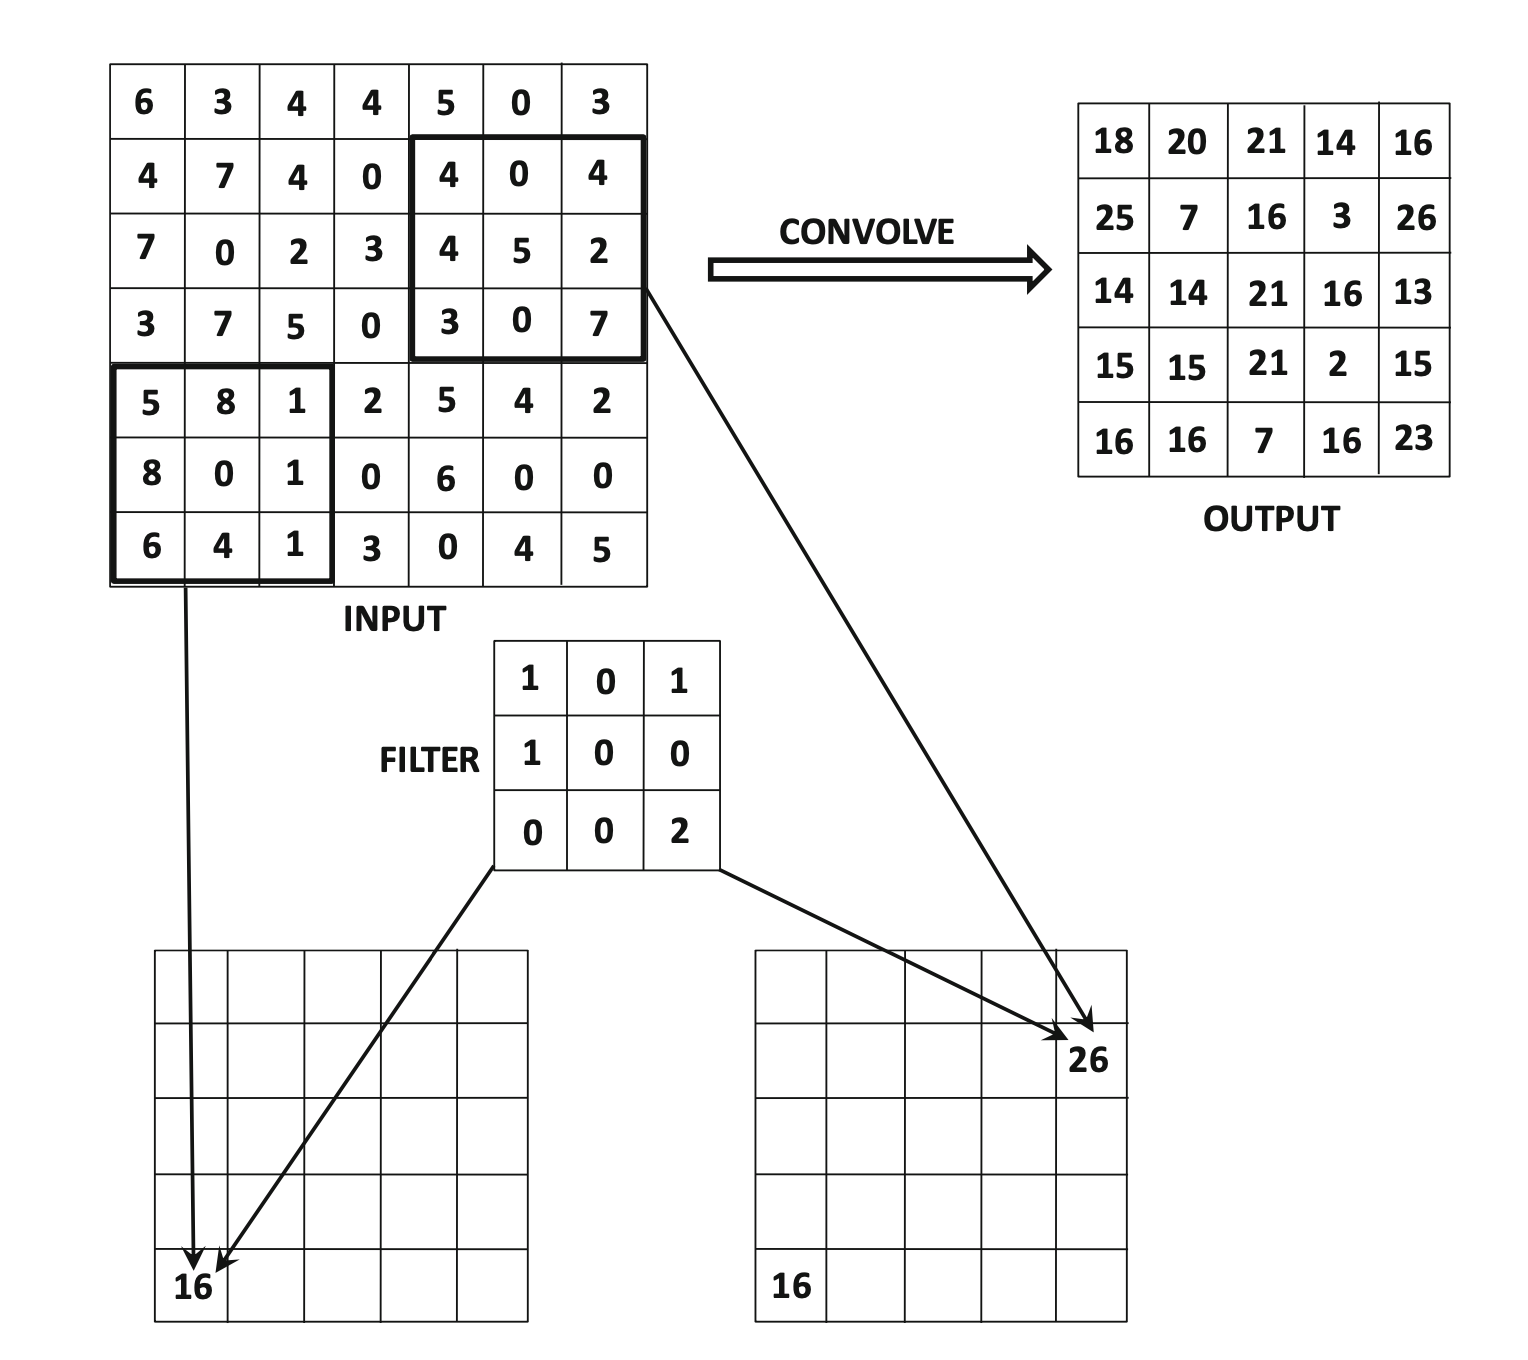
\includegraphics[width=10cm]{kapitel2/conv_layers.png}
    \caption[Die Faltung in einem CNN]{Die Faltungsoperation geschieht durch eine Punktprodukt Operation über des Filters, was über alle räumlichen Positionen wiederholt wird \enquote{Tiefe} sind die 3 Farbkanäle (rot, grün, blau) aus \cite*[321]{Aggarwal2018}.}
    \label{Kap2:Conv}
  \end{figure}

  \subsubsection{Padding}
  Es ist zu beobachtung, dass die Faltungsoperation die Größe der $(q + 1)$-ten Schicht im Vergleich zur Größe der $q$-ten Schicht verringert. Diese Art der Größenreduzierung ist im Allgemeinen nicht wünschenswert, da sie dazu neigt, einige Informationen entlang der Bildränder (oder der Feature-Map im Fall von ausgeblendeten Ebenen) zu verlieren. Dieses Problem kann durch Auffüllen (padding) gelöst werden. Beim Auffüllen werden  \enquote{Pixel} rund um die Ränder der Feature-Map hinzugefügt. Der Wert jedes dieser aufgefüllten Feature-Werte wird auf 0 gesetzt, unabhängig davon, ob die Eingabe oder die ausgeblendeten Ebenen aufgefüllt werden. Diese Bereiche tragen nicht zum endgültigen Punktprodukt bei, da ihre Werte auf 0 gesetzt sind. Ein Teil des Filters aus den Rändern der Schicht wird \enquote{herausragt} und dann durch das Durchführen des Punktprodukts nur über den Teil der Ebene, in dem die Werte definiert sind ersetzt \cite*[323]{Aggarwal2018}.


\subsection{Pooling Layer}
Es ist üblich, regelmäßig eine Pooling-Ebene zwischen aufeinanderfolgenden Conv-Ebenen in eine ConvNet-Architektur einzufügen. Seine Funktion besteht darin, die räumliche Größe der Darstellung schrittweise zu verringern, um die Anzahl der Parameter und die Berechnung im Netzwerk zu verringern und damit auch die Überanpassung zu steuern. Die Pooling-Ebene arbeitet unabhängig mit jedem Tiefenabschnitt der Eingabe und ändert die Größe räumlich mithilfe der MAX-Operation. Die gebräuchlichste Form ist eine Pooling-Ebene mit Filtern der Größe 2x2, die mit einem Schritt (Stride) von 2 Downsamples pro Tiefenscheibe in der Eingabe um 2 entlang der Breite und Höhe angewendet werden, wobei 75\% der Aktivierungen verworfen werden. Jede MAX-Operation würde in diesem Fall maximal 4 Zahlen annehmen. Der \enquote{Volumen} bleibt unverändert \cite*{StanfordUniversityCoursecs231n2018a}.

\begin{figure}[H]
  \centering
  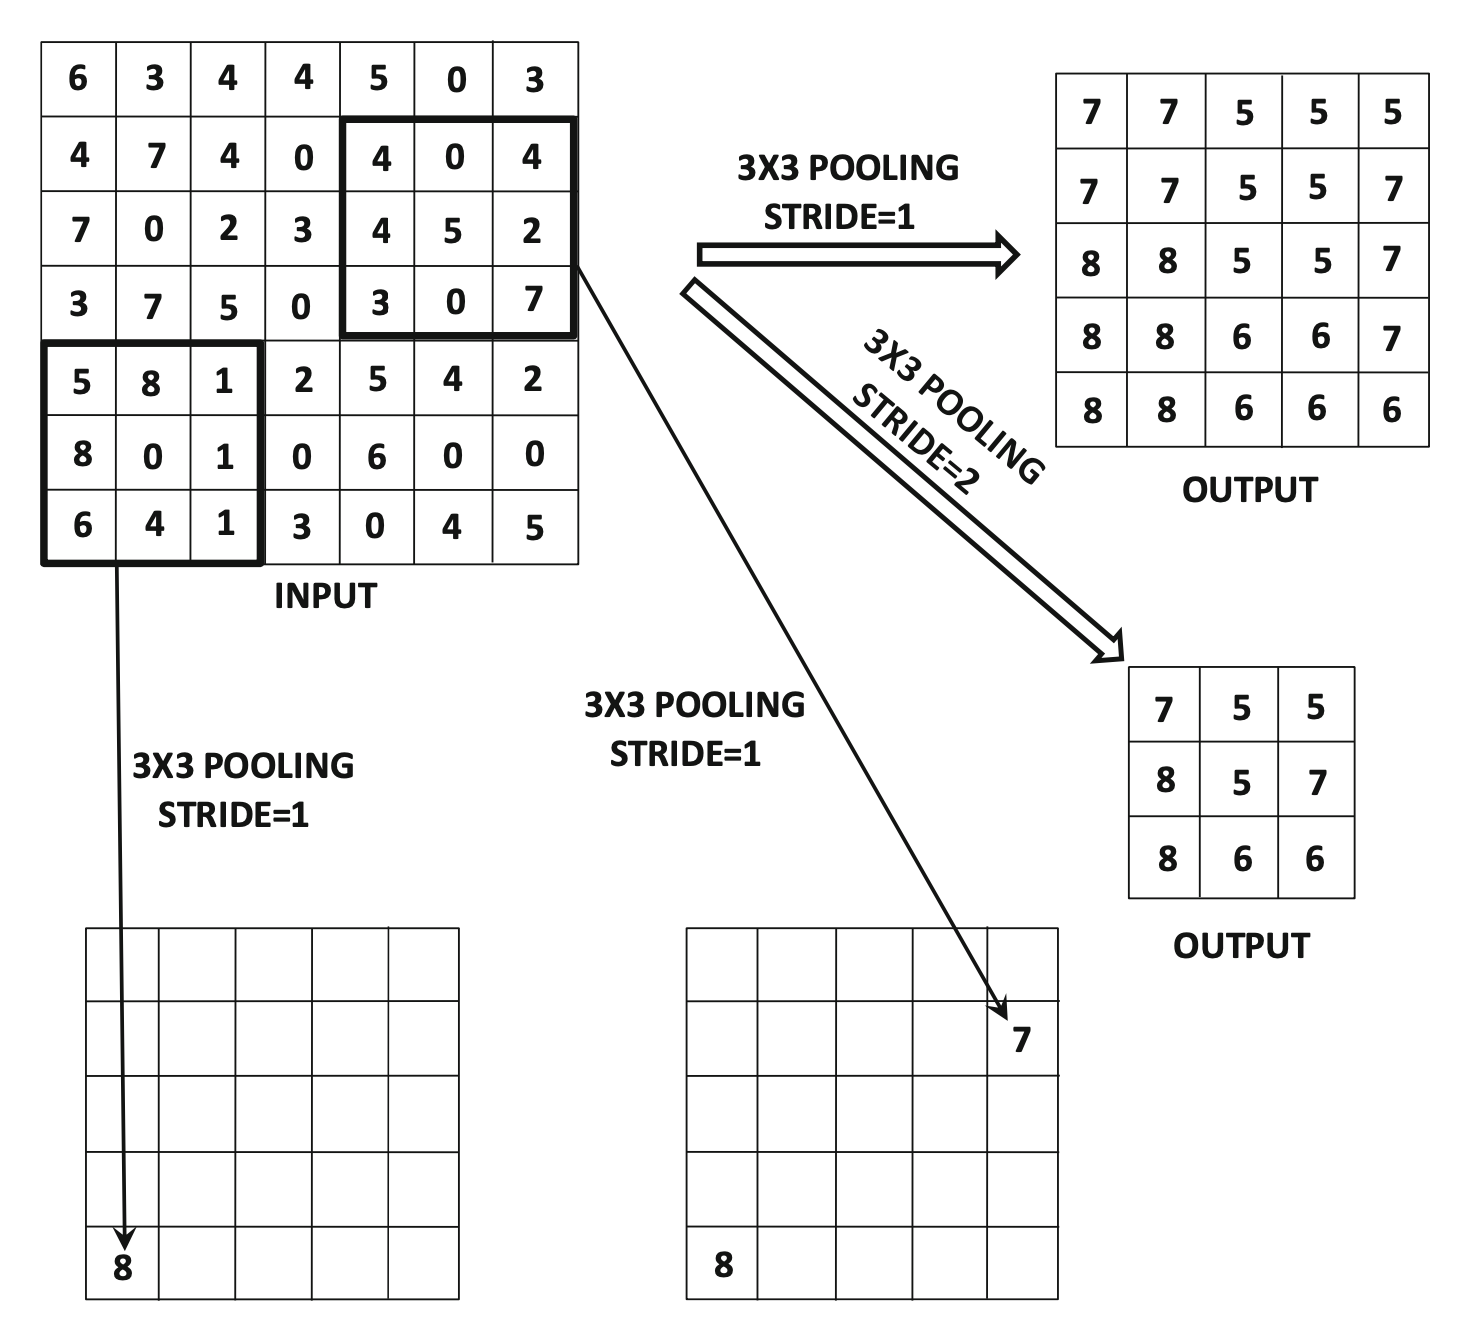
\includegraphics[width=9cm]{kapitel2/maxpooling.png}
  \caption[Max-Pooling]{Ein Beispiel für ein Max-Pooling einer Aktivierungskarte der Größe 7 × 7 mit Stride von 1 und 2. Ein Stride von 1 erzeugt eine 5 × 5-Aktivierungskarte mit stark wiederholten Elementen aufgrund der Maximierung in überlappenden Regionen. Ein Stride von 2 erzeugt eine 3 × 3-Aktivierungskarte mit weniger Überlappung \cite*[326]{Aggarwal2018}.}
  \label{Kap2:Pooling}
\end{figure}


\subsection{Vollständig verbundene Ebenen}
Diese Ebene wird am Ende des Netzwerkes verwendet, um Klassenwerte zu berechnen, die als Ausgabe des Netzwerks dienen sollen. In einem traditionellen vorwärtsgerichteten neuronalen Netzwerk wird jedes Eingangsneuron mit jedem Ausgangsneuron in der nächsten Schicht verbunden. Dies wird auch als vollständig verbundene Schicht bezeichnet. Der einzige Unterschied zwischen FC- und CONV-Schichten besteht darin, dass die Neuronen in der CONV-Schicht nur mit einer lokalen Region in der Eingabe verbunden sind. Die Neuronen in beiden Schichten berechnen jedoch immer noch Punktprodukte, sodass ihre funktionale Form identisch ist. Daher stellt sich heraus, dass es möglich ist, zwischen FC- und CONV-Schichten zu konvertieren \cite*{StanfordUniversityCoursecs231n2018a}.


%   \section{Backpropagation}
%   Wenn vorwärts gerichtetes neuronales Netzwerk (\enquote{feedforward neural network}) verwenden, um eine Eingabe $x$ zu anzunehmen und eine Ausgabe $y$ zu erzeugen, fließen die Informationen durch das Netzwerk vorwärts. Die Eingaben $x$ liefern die initialen Informationen, die sich dann bis zu den verborgenen Einheiten (\enquote{hidden layers}) auf jeder Schicht ausbreiten und schließlich die Ausgabe erzeugen. Dies wird als (\enquote{forward propagation}) bezeichnet. Während des Trainings kann die also die Ausbereitung nach vorne fortgesetzt werden. Der Back-Propagation-Algorithmus \cite*{Rumelhart1986}, oft einfach Backprop genannt, ermöglicht es den Informationen, rückwärts durch das Netzwerk zu fließen \cite[204]{IanGoodfellowYoshuaBengio2016}.

%   Das Herzstück der Backpropagation ist ein Ausdruck aus der partiellen Ableitung, $\partial C$ / $\partial w$ wo die Kostenfunktion $C$ in Bezug auf ein beliebiges Gewicht $w$ (oder einen Bias $b$) im Netzwerk ist. Der Ausdruck sagt uns, wie schnell sich \enquote{die Kosten ändern}, wenn wir die Gewichte und den Bias ändern. Backpropagation gibt uns detaillierte Einblicke, wie das Ändern der Gewichte und des Bias das Gesamtverhalten des Netzwerks verändert \cite*[39]{Nielsen2015}.

% Das Training eines neuronalen Netzwerks bedeutet im Grunde, alle \enquote{Gewichte} zu kalibrieren, indem zwei Schritte wiederholt werden: Forward Pagation und Backpropagation. Beim Forward Pagation wenden wir eine Reihe von Gewichten auf die Eingabedaten an und berechnen eine Ausgabe. Für die erste Forward Pagation werden die Gewichte zufällig ausgewählt. Beim Backpropagation messen wir die Fehlerquote der Ausgabe und passen die Gewichte entsprechend an, um den Fehler zu verringern. Neuronale Netze wiederholen sowohl die Forward Pagation als auch die Backpropagation, bis die Gewichte kalibriert sind, um eine Ausgabe genau vorherzusagen \cite{Miller}.

% Durch Forward Pagation machen neuronale Netze also Vorhersagen. Eingabedaten werden Schicht für Schicht durch das Netzwerk an die letzte Schicht weitergeleitet, die eine Vorhersage ausgibt. Die Ziele der Backpropagation sind das Anpassen jedes Gewicht im Netzwerk proportional dazu, wie viel es zum Gesamtfehler beiträgt. Wenn wir den Fehler jedes Gewichts iterativ reduzieren, haben wir schließlich eine Reihe von Gewichten, die gute Vorhersagen liefern.


% \section{Formelsatz}

% Eine Formel gefällig? Mitten im Text $a_2 = \sqrt{x^3}$ oder als eigener Absatz (siehe Formel~\ref{Formel}):




% Das Aufkommen von Online-Nachrichtenagenturen und die Explosion der Anzahl der Benutzer, die Nachrichten mit diesem Medium konsumieren, haben dazu geführt, dass mehrere Webseiten miteinander konkurrieren, um die Aufmerksamkeit der Benutzer zu erregen. Dies hat dazu geführt, dass Verkaufsstellen kreative Wege geschaffen haben, um Leser auf ihre Website zu locken. Eine der am häufigsten verwendeten Techniken ist die Verwendung von Clickbait-Überschriften. Diese Überschriften wurden speziell dafür entwickelt, um das Interesse des Lesers an dem zu wecken, was versprochen wird. Wenn auf den Artikel geklickt wird jedoch, liefert dieser Artikel normalerweise nicht den Inhalt, den der Leser Ursprüngich gesucht hat. In den Abbildungen \ref{Kap2:ClickBait} und \ref{Kap2:News}\footnote{Entnommen aus: https://github.com/MichaelGoodale/Clickbait-Classifier} wird der Unterschied zwischen Clickbaits und \enquote{normalen} Nachrichten aufgezeigt.

% \begin{figure}
%   \centering
%   \includegraphics[width=12cm]{kapitel2/clickbait.png}
%   \caption[Beispiel von Clickbait]{Beispiel von Clickbait}
%   \label{Kap2:ClickBait}
% \end{figure}


% \begin{figure}[ht]
%   \centering
%   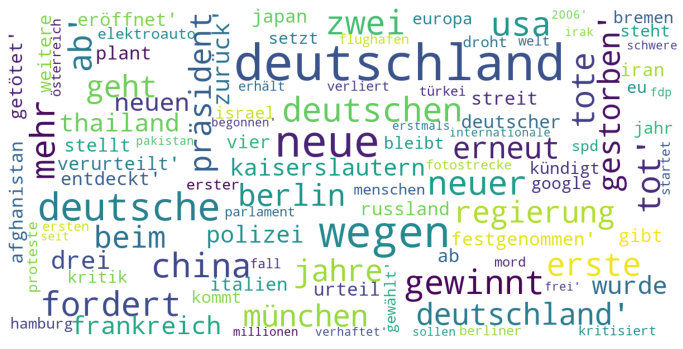
\includegraphics[width=12cm]{kapitel2/news.png}
%   \caption[Beispiel von \enquote{normalen} Nachrichten]{Beispiel von \enquote{normalen} Nachrichten}
%   \label{Kap2:News}
% \end{figure}


% \section{Lösungsansatz}
% Textklassifizierung ist eine gängige Art, wie man \enquote{gute} von \enquote{bösen} Texten unterscheiden kann. Es ist allerdingt nicht praktisch ein großes Sprachmodell wie GPT-3 Browserkompatible zu machen. Erstens ist es völlig \enquote{overkill} für ein solches Problem ein Sprachmodell zu benutzen und zweitens passen diese großen Modelle nicht in den Browser, da die Ladezeit nicht praktisch ist.

% Mit dieser Arbeit möchte ich ein Modell erstellen, um Clickbait Überschriften zu erkennen. Es wäre Hilfreich, wenn es ein Dienst gibt, welches eine Überschrift liest und dem Benutzer vorhersagt, ob es sich um Clickbait handelt oder nicht. So kann der Nutzer seine Zeit sparen und muss nicht auf die Seite gehen. Das Hauptprodukt ist dabei dieser Dienst, welches ganz einfach in jede HTML-Seite importiert werden kann. Dieser Dienst muss klein und schnell und gute dabei möglichst Ergebnisse liefern.

% \section{Aufbau der Arbeit}


% Im Abschnitt 2.6 Grobgliederung befindet sich eine mögliche Gliederung für diese Arbeit, auf die ich verweisen möchte. Zunächst wird in den Kapiteln 2 und 3 eine theoretische Grundlage geschaffen. Diese Kapitel beschäftigen sich mit Deep Learning und den mathematisch/statistschischen Erklärungen. Kapitel 3 orientiert sich eher mit NLP und insbesondere mit Worteinbettungen und wie moderne Computer die natürliche Sprache verstehen. Kapitel 4 soll den aktuellen Forschungsstand mit meiner Arbeit vergleichen. Es sollen verwandte Lösungsansätze kategorisch analysiert werden.

% Um mit dem eigentlichen Kern anzufangen, benötigt diese Arbeit an Daten. In Kapitel 5 wird gezeigt wie mittelt Webscraping. Dieser Datensatz wird händisch gelabelt und besteht aus einem Titel und einer Klasse. Die erste erste hälfte des Datensatzes wird aus Wikinews\footnote{https://de.wikinews.org/wiki/Hauptseite} geladen. Wikinews hat einen API-Zugang wodurch Nachrichten, welche nicht Clickbait sind in den Datensatz gebracht werden können. Ich habe dafür bereits mehr als 10.000 Nachrichten-Titel in eine Datenbank geladen. Die zweite hälfte des Datensatzes wird mittels Webseiten mit Scrapy\footnote{ https://scrapy.org/} gescraped. Die ersten 1.000 Titel sind bereits in die Datenbank\footnote{https://github.com/youurt/klickkoeder/blob/main/klickscraper/klickscraper.db} geladen worden.

% Nachdem ausreichend Daten geladen werden, ist geplant diese Daten zu laben. Damit später keine Verzerrungen bei den Daten entstehen, plane ich noch eine weitere Person zum Unterstützen beim Labeln mit in die Arbeit zu nehmen. Dieses wird mit dem Betreuer der Arbeit noch abgeklärt werden müssen. Der restliche Teil dieses Kapitels beschäftigt sich mit der Analyse der Daten um bestimmte Muster zu erkennen und die Daten in ein passendes Format zu bringen.

% Ich werde ein Modell in TensorFlow.js entwickeln. Dieses Modell soll möglichst klein sein und schnell sein. Um mit TensorFlow.js arbeiten zu können muss der Text in Vektoren umgewandelt werden.

% Mit einem Versuchsaufbau soll das Modell getestet und analysiert werden. Schließlich soll das Modell in die Browser-Umgebung gebracht und mittels eines minimalistischen React Frontends angeboten werden.

% \begin{figure}[ht]
%   \centering
%   \includegraphics[width=12cm]{kapitel2/beispiel.png}
%   \caption[Beispiel einer Systemarchitektur]{Beispiel einer Systemarchitektur entnommen aus \cite{cho2019shop}. Der Client bekommt beim laden der Seite, neben dem HTML, CSS und dem JavaScript, welches für das Frontend nötig ist, ein weiteres Script, welches die TensorFlow.js API bereitstellt. Die Berechnung findet im Browser, beim Client statt, wo auch das Modell sich befindet.}
%   \label{Kap2:SystemArchitektur}
% \end{figure}

% \section{Wissenschaftlicher Beitrag}
% \begin{itemize}
%   \item Den Stand der Technik in Bezug auf Deep Learning und Worteinbettungen zeigen
%   \item Erstellung und labeln eines Datensatzes für deutsche Clickbaits
%   \item Implementierung eines NLP-Problemes im Browser ohne zusätzliche Software oder Plugins, mit TensorFlow.js
%   \item Optimierung des Browsers für Deep Learning
%   \item Auswahl des optimalen Modells und der Trainingsmethode
%   \item Produktion eines Dienstes, um Clickbait Nachrichten vorzubeugen
% \end{itemize}

% \section{Einstiegsliteratur}

% \begin{itemize}
%   \item \cite{Kaur2020a}
%   \item \cite{Chavan2019}
%   \item \cite{vorakitphan2018clickbait}
%   \item \cite{Anand2017}
%   \item \cite{gairola2017neural}
%   \item \cite{kumar2018identifying}
%   \item \cite{glenski2017fishing}
%   \item \cite{chawda2019novel}
%   \item \cite{seopredicting}
%   \item \cite{cho2019shop}
%   \item \cite{roberts2018magenta}
%   \item \cite{aggarwal2012survey}
%   \item \cite{kowsari2019text}
%   \item \cite{korde2012text}
%   \item \cite{altinel2018semantic}
%   \item \cite{nordberg2020crucial}
%   \item \cite{raamkumar2020use}
%   \item \cite{rivera2020identifying}
%   \item \cite{nguyen2020real}
%   \item \cite{zhang2015character}
%   \item \cite{kiranyaz20191d}
%   \item \cite{severyn2015unitn}
%   \item \cite{severyn2015twitter}
%   \item \cite{zhao2019speech}
%   \item \cite{eren2019generic}
% \end{itemize}

% \section{Grobgliederung}
% \renewcommand{\labelenumii}{\theenumii}
% \renewcommand{\theenumii}{\theenumi.\arabic{enumii}.}

% \begin{enumerate}

%   \item Einleitung
%         \begin{enumerate}
%           \item Motivation
%           \item Wissenschaftlicher Beitrag
%           \item Struktur der Arbeit
%         \end{enumerate}

%   \item Neuronale Netze
%         \begin{enumerate}
%           \item Einleitung
%           \item Arten des Neuronalen Lernens
%           \item Netzwerkparameter und Hyperparameter
%           \item Aktivierungsfunktionen
%           \item Verlustfunktion
%           \item Optimizer
%           \item Epochen
%           \item TensorFlow.js
%           \item Schluss
%         \end{enumerate}

%   \item Die natürliche Sprache
%         \begin{enumerate}
%           \item Einleitung
%           \item Vektorisierung des Textes durch Encoding
%           \item Worteinbettungen
%           \item 1d CNN
%           \item Schluss
%         \end{enumerate}

%   \item Aktueller Forschungsstand
%         \begin{enumerate}
%           \item Einleitung
%           \item Clickbaits und Deep Learning Ansätze
%           \item TensorFlow.js
%           \item Worteinbettungen
%         \end{enumerate}

%   \item Korpuskonstruktion und Analyse
%         \begin{enumerate}
%           \item Einleitung
%           \item Rohdatenerhebung mittels Webscraping
%           \item Das labeln der Daten
%           \item Explorative Datenanalyse
%           \item Vorverarbeitung der Daten
%           \item Schluss
%         \end{enumerate}

%   \item Methodik
%         \begin{enumerate}
%           \item Einleitung
%           \item Die Systemarchitektur
%           \item JavaScript
%           \item Modelling
%           \item Einbettung in das Frontend
%           \item Schluss
%         \end{enumerate}

%   \item Versuchsaufbau und Diskussion der Ergebnisse
%         \begin{enumerate}
%           \item Einleitung
%           \item Anpassung der Netzwerkparameter und Hyperparameter
%           \item Leistungsmessungen
%           \item Vergleich und Darstellung der Ergebnisse
%           \item Schluss
%         \end{enumerate}

%   \item Schluss
%         \begin{enumerate}
%           \item Fazit zum Forschungsbeitrag
%           \item Abschließende Gedanken
%           \item Zukunft der Arbeit
%         \end{enumerate}
% \end{enumerate}




% \section{Hervorhebungen}
% \label{Einleitung:Textauszeichnungen}

% Achten Sie bitte auf die grundlegenden Regeln der Typographie\index{Typographie}\footnote{Ein Ratgeber in allen Detailfragen ist \cite{Forssman2002}.}, wenn Sie Ihren Text schreiben. Hierzu gehören z.\,B. die Verwendung der richtigen "`Anführungszeichen"' und der Unterschied zwischen Binde- (-), Gedankenstrich (--) und langem Strich (---). Sie erhalten den Bindestrich in \LaTeX{} mit \verb+-+, den Gedankenstrich mit \verb+--+ und den langen Strich mit \verb+---+.

% Wenn Sie Text hervorheben wollen, dann setzten Sie ihn mit \verb+\textit+ \textit{kursiv} (Italic) und nicht \textbf{fett} (Bold). Fettdruck ist Überschriften vorbehalten; im Fließtext stört er den Lesefluss. Das \underline{Unterstreichen} von Fließtext ist im gesamten Dokument tabu und kann maximal bei Pseudo"=Code vorkommen.\index{Hervorhebungen}


% \section{Anführungszeichen}

% Deutsche Anführungszeichen werden mit \verb+"`+ und \verb+"'+ erzeugt: "`dieser Text steht in \glq Anführungszeichen\grq; alles klar?"'. Englische Anführungszeichen hingegen mit \verb+``+ und \verb+''+: ``this is an `English' quotation''. Beachten Sie, dass Sie in Zitaten immer die zur Sprache passenden Anführungszeichen verwenden. Die Verwendung von \verb+"+ ist für Anführungszeichen immer falsch und führt bei \LaTeX{} zu seltsamen "Effekten".

% Um sich diesen Ärger zu sparen, biete sich die Verwendung des Paketes \textit{csquotes} und des Kommandos \verb+\enquote+ an. Hierdurch werden die Anführungszeichen korrekt für die eingestellte Sprache gesetzt und Sie müssen sich \enquote{keine Sorgen mehr über die \enquote{Anführungszeichen} machen}.


% \section{Abkürzungen}
% \index{Abkürzungen}
% \index{Abbreviation|see{Abkürzungen}}

% Eine \ac{ABK} (\verb+\ac{ABK}+) wird bei der ersten Verwendung ausgeschrieben. Danach nicht mehr: \ac{ABK}. Man kann allerdings mit \verb+\acl+ die Langform explizit anfordern (\acl{ABK}) oder mit \verb+\acs+ die Kurzform (\acs{ABK}) oder mit \verb+\acf+ auch noch einmal die Definition (\acf{ABK}).

% Beachten Sie, dass bei Abkürzungen, die für zwei Wörter stehen, ein kleines Leerzeichen nach dem Punkt kommt: z.\,B. bzw. \zb{} und d.\,h. bzw. \dahe{}. Das Template bietet hierfür die beiden Makros \verb+\zb{}+ und \verb+\dahe{}+.


% \section{Querverweise}

% Querverweise auf eine Kapitelnummer macht man im Text mit \verb+\ref+ (Kapitel~\ref{Einleitung:Textauszeichnungen}) und auf eine bestimmte Seite mit \verb+\pageref+ (Seite~\pageref{Einleitung:Textauszeichnungen}). Man kann auch den Befehl \verb+\autoref+ benutzen, der automatisch die Art des referenzierten Elements bestimmt (\zb{} \autoref{Einleitung:Textauszeichnungen} oder \autoref{Kap2:Kopplungsformen}).


% \section{Fußnoten}

% Fußnoten werden einfach mit in den Text geschrieben und zwar genau an die Stelle\footnote{An der die Fußnote auftauchen soll}. Hierzu dient der Befehl \verb+\footnote{Text}+.


% \section{Tabellen}

% Tabellen werden normalerweise ohne vertikale Striche gesetzt, sondern die Spalten werden durch einen entsprechenden Abstand voneinander getrennt.\footnote{Siehe \cite[S. 89]{Willberg1999}.} Zum Einsatz kommen ausschließlich horizontale Linien (siehe Tabelle~\ref{Kap2:Kopplungsformen}).

% \begin{table}[h]
%   \caption{Ebenen der Kopplung und Beispiele für enge und lose Kopplung}
%   \label{Kap2:Kopplungsformen}
%   \renewcommand{\arraystretch}{1.2}
%   \centering
%   \sffamily
%   \begin{footnotesize}
%     \begin{tabular}{l l l}
%     \toprule
%     \textbf{Form der Kopplung} & \textbf{enge Kopplung} & \textbf{lose Kopplung}\\
%     \midrule
%     Physikalische Verbindung	&	Punkt-zu-Punkt	& 	über Vermittler\\
%     Kommunikationsstil	&	synchron		&	asynchron\\
%     Datenmodell	&	komplexe gemeinsame Typen	&	nur einfache gemeinsame Typen\\
%     Bindung	&	statisch		&	dynamisch\\
%     \bottomrule
%     \end{tabular}
%   \end{footnotesize}
%   \rmfamily
% \end{table}

% Eine Tabelle fließt genauso, wie auch Bilder durch den Text. Siehe Tabelle~\ref{Kap2:Kopplungsformen}.

% Manchmal möchte man Tabellen, in denen der Text in der Tabellenspalte umbricht. Hierzu dient die Umgebung \texttt{tabularx}, wobei \texttt{L} eine Spalte mit Flattersatz und \texttt{X} eine mit Blocksatz definiert. Die Breite der Tabelle kann über den Faktor vor \verb+\textwidth+ angegeben werden.

% \begin{table}[h]
%   \caption{Teildisziplinen der Informatik}
%   \label{Kap2:Teildisziplinen}
%   \renewcommand{\arraystretch}{1.2}
%   \centering
%   \sffamily
%   \begin{footnotesize}
%     \begin{tabularx}{0.9\textwidth}{l X L}
%       \toprule
%       \textbf{Gebiet} & \textbf{Definition} & \textbf{Beispiel}\\
%       \midrule
%       \emph{Praktische Informatik} & Informatik-Disziplinen, welche sich vorwiegend mit der Entwicklung und Anwendung der Software-Komponenten befassen & Programmentwicklung, Compilerbau; im Aufbau von z.B. Informationssystemen und Netzwerken ergeben sich Überlappungen mit der technischen Informatik \\
%       \emph{Technische Informatik} & Informatik-Disziplinen, welche sich vorwiegend mit der Entwicklung und Anwendung der Hardware-Komponenten befassen & Digitaltechnik, Mikroprozessortechnik \\
%       \emph{Theoretische Informatik} & Informatik-Disziplinen, welche sich mit der Entwicklung von Theorien und Modellen der Informatik befassen und dabei viel Substanz aus der Mathematik konsumieren & Relationenmodell, Objekt-Paradigmen, Komplexitätstheorie, Kalküle \\
%       \emph{Angewandte Informatik} & Informatik als instrumentale Wissenschaft & Rechtsinformatik, Wirtschaftsinformatik, Geoinformatik \\
%       \bottomrule
%     \end{tabularx}
%   \end{footnotesize}
%   \rmfamily
% \end{table}


% \section{Harveyballs}

% \begin{quote}
%     Harvey Balls sind kreisförmige Ideogramme, die dazu dienen, qualitative Daten anschaulich zu machen. Sie werden in Vergleichstabellen verwendet, um anzuzeigen, inwieweit ein Untersuchungsobjekt sich mit definierten Vergleichskriterien deckt. \parencite{Wikipedia_HarveyBalls}
% \end{quote}

% \begin{table}[h]
%   \caption{Beispiel für Harvey Balls}
%   \label{tab:harveyexample}
%   \centering
%   \begin{tabular}{lccc}
%     \toprule
%     & Ansatz 1 & Ansatz 2 & Ansatz 3\\
%     \midrule
%     Eigenschaft 1	& \harveyBallNone & \harveyBallQuarter & \harveyBallHalf \\
%     Eigenschaft 2	& \harveyBallHalf & \harveyBallThreeQuarter & \harveyBallFull \\
%     Eigenschaft 3	& \harveyBallFull & \harveyBallThreeQuarter & \harveyBallQuarter\\
%     \bottomrule
%   \end{tabular}
% \end{table}


% \section{Aufzählungen}

% Aufzählungen sind toll.

% \begin{itemize}
%   \item Ein wichtiger Punkt
%   \item Noch ein wichtiger Punkt
%   \item Ein Punkt mit Unterpunkten
%     \begin{itemize}
%       \item Unterpunkt 1
%       \item Unterpunkt 2
%     \end{itemize}
%   \item Ein abschließender Punkt ohne Unterpunkte
% \end{itemize}


% Aufzählungen mit laufenden Nummern sind auch toll.

% \begin{enumerate}
%   \item Ein wichtiger Punkt
%   \item Noch ein wichtiger Punkt
%   \item Ein Punkt mit Unterpunkten
%     \begin{enumerate}
%       \item Unterpunkt 1
%       \item Unterpunkt 2
%     \end{enumerate}
%   \item Ein abschließender Punkt ohne Unterpunkte
% \end{enumerate}
